\documentclass[12pt, letterpaper]{article}
%\setlength{\parindent}{0in}
\setlength{\textheight}{8.9in}
\setlength{\textwidth}{6.8in}
\setlength{\oddsidemargin}{-0.3in}
\setlength{\evensidemargin}{0.0in}
\addtolength{\topmargin}{-1in}
\setlength{\parskip}{0.1in}

\usepackage{amsmath, amsfonts}
\usepackage{graphicx}
\usepackage{caption}
\usepackage{subcaption}

\usepackage{url}
\usepackage{multirow}
\usepackage{setspace}
\onehalfspacing

\newcommand{\bmeta}{\boldsymbol{\eta}}
\newcommand{\bmtheta}{\boldsymbol{\theta}}
\newcommand{\bmbeta}{\boldsymbol{\beta}}
\newcommand{\bmphi}{\boldsymbol{\phi}}
\newcommand{\bmpi}{\boldsymbol{\pi}}
\newcommand{\bmxi}{\boldsymbol{\xi}}
\newcommand{\bmnu}{\boldsymbol{\nu}}
\newcommand{\bmmu}{\boldsymbol{\mu}}
\newcommand{\bmalpha}{\boldsymbol{\alpha}}
\newcommand{\bmzeta}{\boldsymbol{\zeta}}
\newcommand{\bmgamma}{\boldsymbol{\gamma}}
\newcommand{\bmomega}{\boldsymbol{\omega}}

\newcommand{\bmY}{\mathbf{Y}}
\newcommand{\bmZ}{\mathbf{Z}}
\newcommand{\bmX}{\mathbf{X}}
\newcommand{\bmV}{\mathbf{V}}
\newcommand{\bmW}{\mathbf{W}}
\newcommand{\bmU}{\mathbf{U}}
\newcommand{\bmR}{\mathbf{R}}
\newcommand{\bmS}{\mathbf{S}}
\newcommand{\bmb}{\mathbf{b}}

\newcommand{\bmM}{\mathbf{M}}
\newcommand{\bmSigma}{\boldsymbol{\Sigma}}
\newcommand{\bmI}{\mathbf{I}}
\newcommand{\bmTheta}{\boldsymbol{\Theta}}


\newcommand{\bea}{\begin{eqnarray}} 
\newcommand{\eea}{\end{eqnarray}} 
\newcommand{\beas}{\begin{eqnarray*}} 
\newcommand{\eeas}{\end{eqnarray*}} 
\newcommand{\benum}{\begin{enumerate}} 
\newcommand{\eenum}{\end{enumerate}} 
\newcommand{\bd}{\begin{description}}
\newcommand{\ed}{\end{description}}
\newcommand{\bi}{\begin{itemize}}
\newcommand{\ei}{\end{itemize}}

\newcommand{\mydots}{...}

\usepackage{color}
\usepackage{xcolor}

\definecolor{mygreen}{rgb}{0,0.75,0}
\definecolor{mypurple}{rgb}{0.7,0,0.8}

\newcommand{\shade}[1]{\colorbox{gray}{#1}}
\newcommand{\highlight}[1]{\colorbox{yellow}{#1}}
\newcommand{\gbox}[1]{\colorbox{green}{#1}}
\newcommand{\tcr}[1]{\textcolor{red}{#1}}
\newcommand{\tcg}[1]{\textcolor{mygreen}{#1}}
\newcommand{\tcb}[1]{\textcolor{blue}{#1}}
\newcommand{\tcp}[1]{\textcolor{mypurple}{#1}}
\newcommand{\tcbk}[1]{\textcolor{black}{#1}}

\begin{document}

\begin{center}
\large Prediction Model for Active Surveillance of Prostate Cancer\\
R Yates Coley, Scott Zeger, Aaron Fisher,  Ken Pienta, H Ballentine Carter \\\textit{(can discuss inclusion, order)} \\
July 6, 2015\\
\end{center}



\section{Introduction}
Prostate cancer is the most commonly diagnosed non-skin cancer in men in the United States \cite{SEER2014}. Upon diagnosis, early curative treatment with surgery, radiation, or androgen deprivation therapy is common \cite{Cooperberg2010,Welch2009}. Prostate cancer treatments can be physically, emotionally, and financially taxing for patients. In particular, one-month mortality after surgery is as high as 0.5$\%$, and at least 20-30$\%$ of men experience urinary incontinence and erectile dysfunction after surgery or radiotherapy \cite{Chou2011a,Chou2011b}. 

Active surveillance with curative intent offers an alternative to early treatment for individuals with lower risk disease detected \cite{Carter2007, Khatami2007, Klotz2010, Soloway2008, Tosoian2011, vanAs2008, vandenBergh2009}. Though active surveillance regimes vary, the approach generally entails regular biopsies (e.g., annually) with curative intervention recommended upon detection of higher risk histological features, as determined by the Gleason grading system. Biopsies with a Gleason score of 6 indicate low risk disease while a Gleason score of 7 or above is considered \textit{reclassification} to a higher risk. Prostate-specific antigen (PSA) is also routinely measured and may be used to recommend biopsies. 

The success of active surveillance programs depend on clinicians' ability to identify tumors with metastatic potential with sufficient time for curative intervention to be effective. Biopsies used to characterize tumors, however, are only informative about the sampled tissue and, moreover, have imperfect sensitivity and specificity\cite{Epstein2012}. As a result, biopsy results do not indicate the true state of an individual's cancer, but rather are measurements made with error. Existing clinical support tools that predict biopsy outcomes for active surveillance patients, including, most recently, Ankerst et al. 2015\nocite{Ankerst2015}, contribute valuable information to guide decisions about biopsy timing and frequency but are insufficient to address patients' primary concerns. Instead, patients and clinicians would prefer prediction of the pathological make-up of the entire prostate, including any presence of higher risk features, in order to guide decision-making.

With this motivation in mind, we have developed a Bayesian hierarchical model that enables prediction of an individual's underlying disease status via joint modeling of repeated PSA measurements and biopsies. Specifically, we predict a binary cancer state- \textit{indolent} or \textit{aggressive}- with the latter defined as a true (i.e., measured without error) Gleason score of 7 or higher. Predictions are informed by a subset of patients for whom the true state is observed, that is, patients who underwent elective prostatectomy (either before of after reclassification) and for whom results of the pathological analysis of the removed tissue is available. In this sense, cancer state operates as a partially-latent class in the proposed model \cite{Wu2015}. 

As reflected through a joint modeling framework, an individual's cancer state influences both the level and trajectory of PSA measurements as well as the outcome of repeated biopsies. These relationships are illustrated by the directed acyclic graph (DAG) in Figure 1(a) for a single point in time and in Figure 1(b) for multiple time points. In the model we are proposing, PSA measurements follow a mixed effects model with mean effects varying across latent classes \cite{Laird1982}. Then, biopsy outcomes, a binary indicator of reclassification at each year of follow-up, are modeled with a pooled logistic regression model under the assumption that biopsy results are independent conditional on cancer state and covariates (age, time since diagnosis, etc.)\cite{Cupples1988,D'Agostino1990}. As codified in the Figure 1(b) DAG, PSA and biopsy results are also assumed to be conditionally independent given latent class. 

\begin{figure}
\begin{center}
\begin{subfigure}[b]{0.3\textwidth}
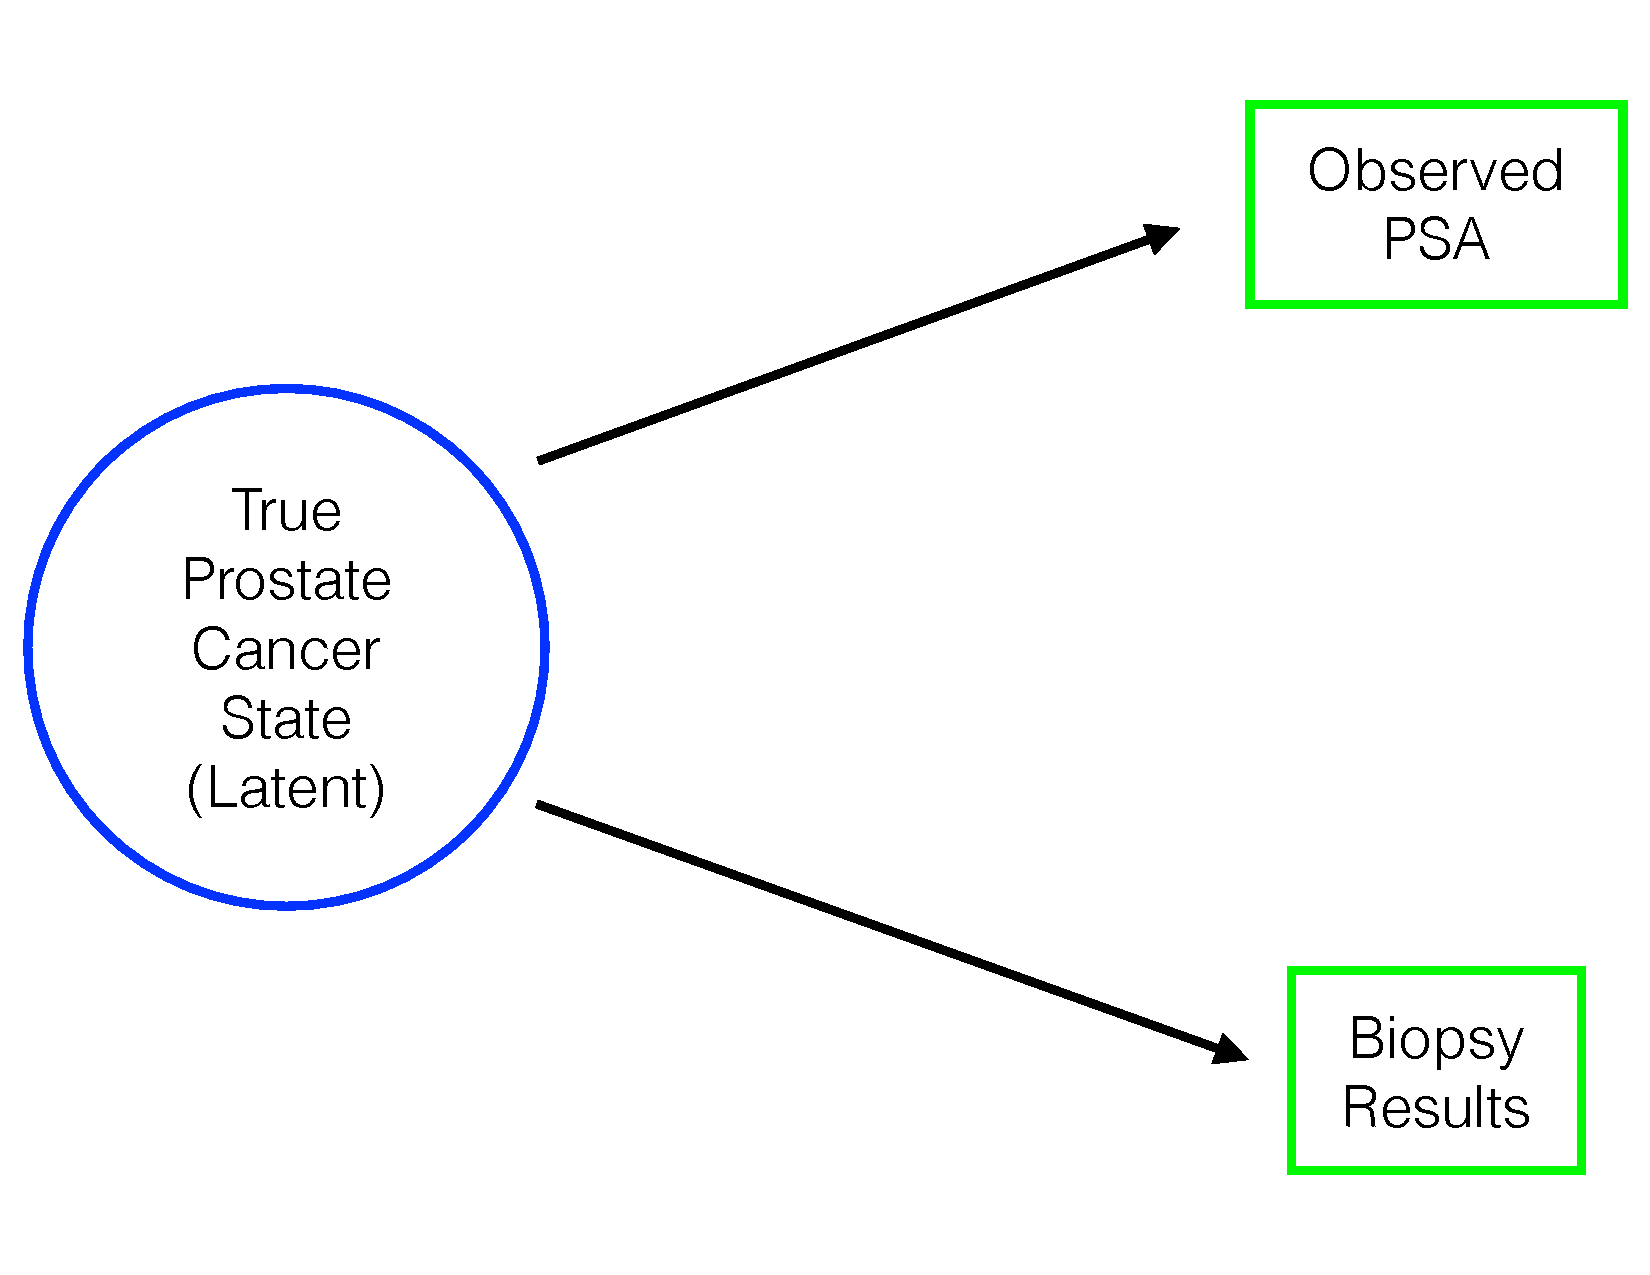
\includegraphics[width=\textwidth]{dag1}
\caption{}%Time Point Joint Model}
\label{fig:dag1}
\end{subfigure}
\begin{subfigure}[b]{0.3\textwidth}
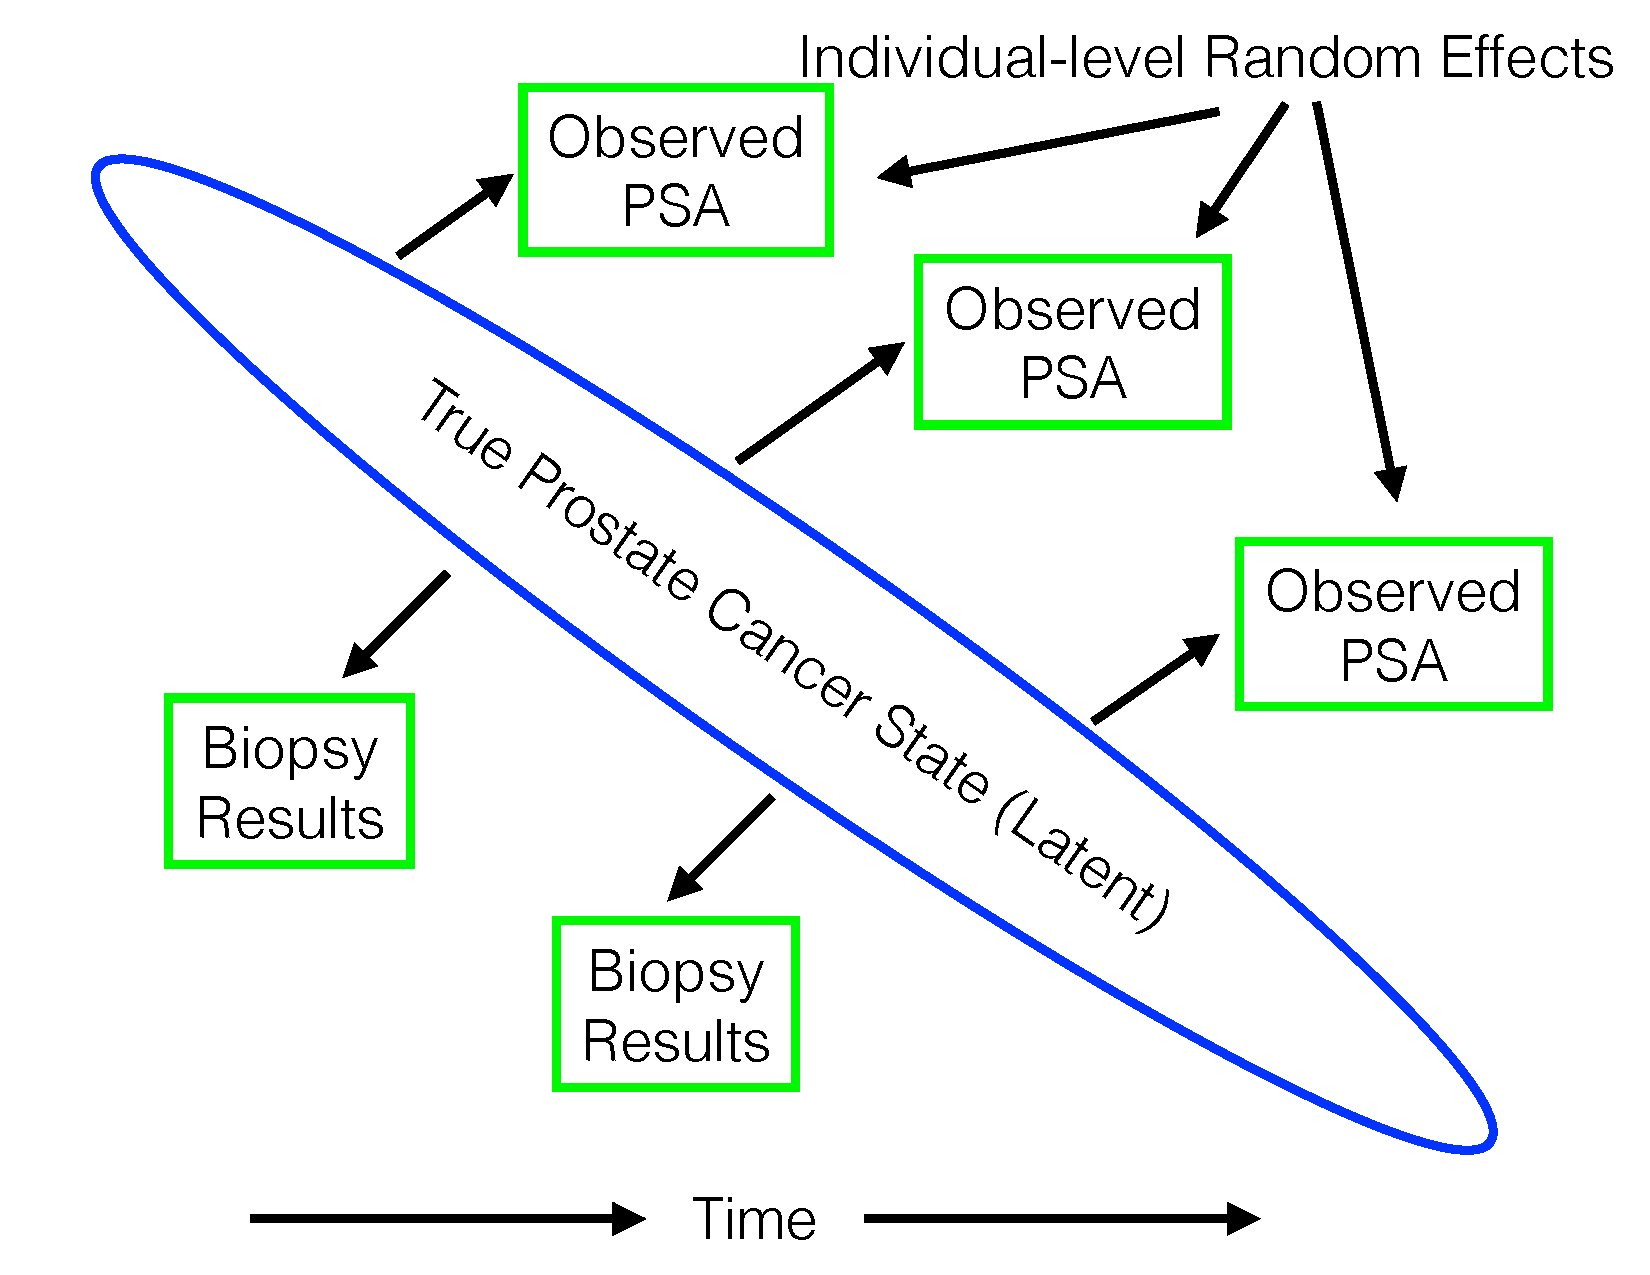
\includegraphics[width=\textwidth]{dag2}
\caption{}%Time-Varying Joint Model}
\label{fig:dag2}
\end{subfigure}
\begin{subfigure}[b]{0.3\textwidth}
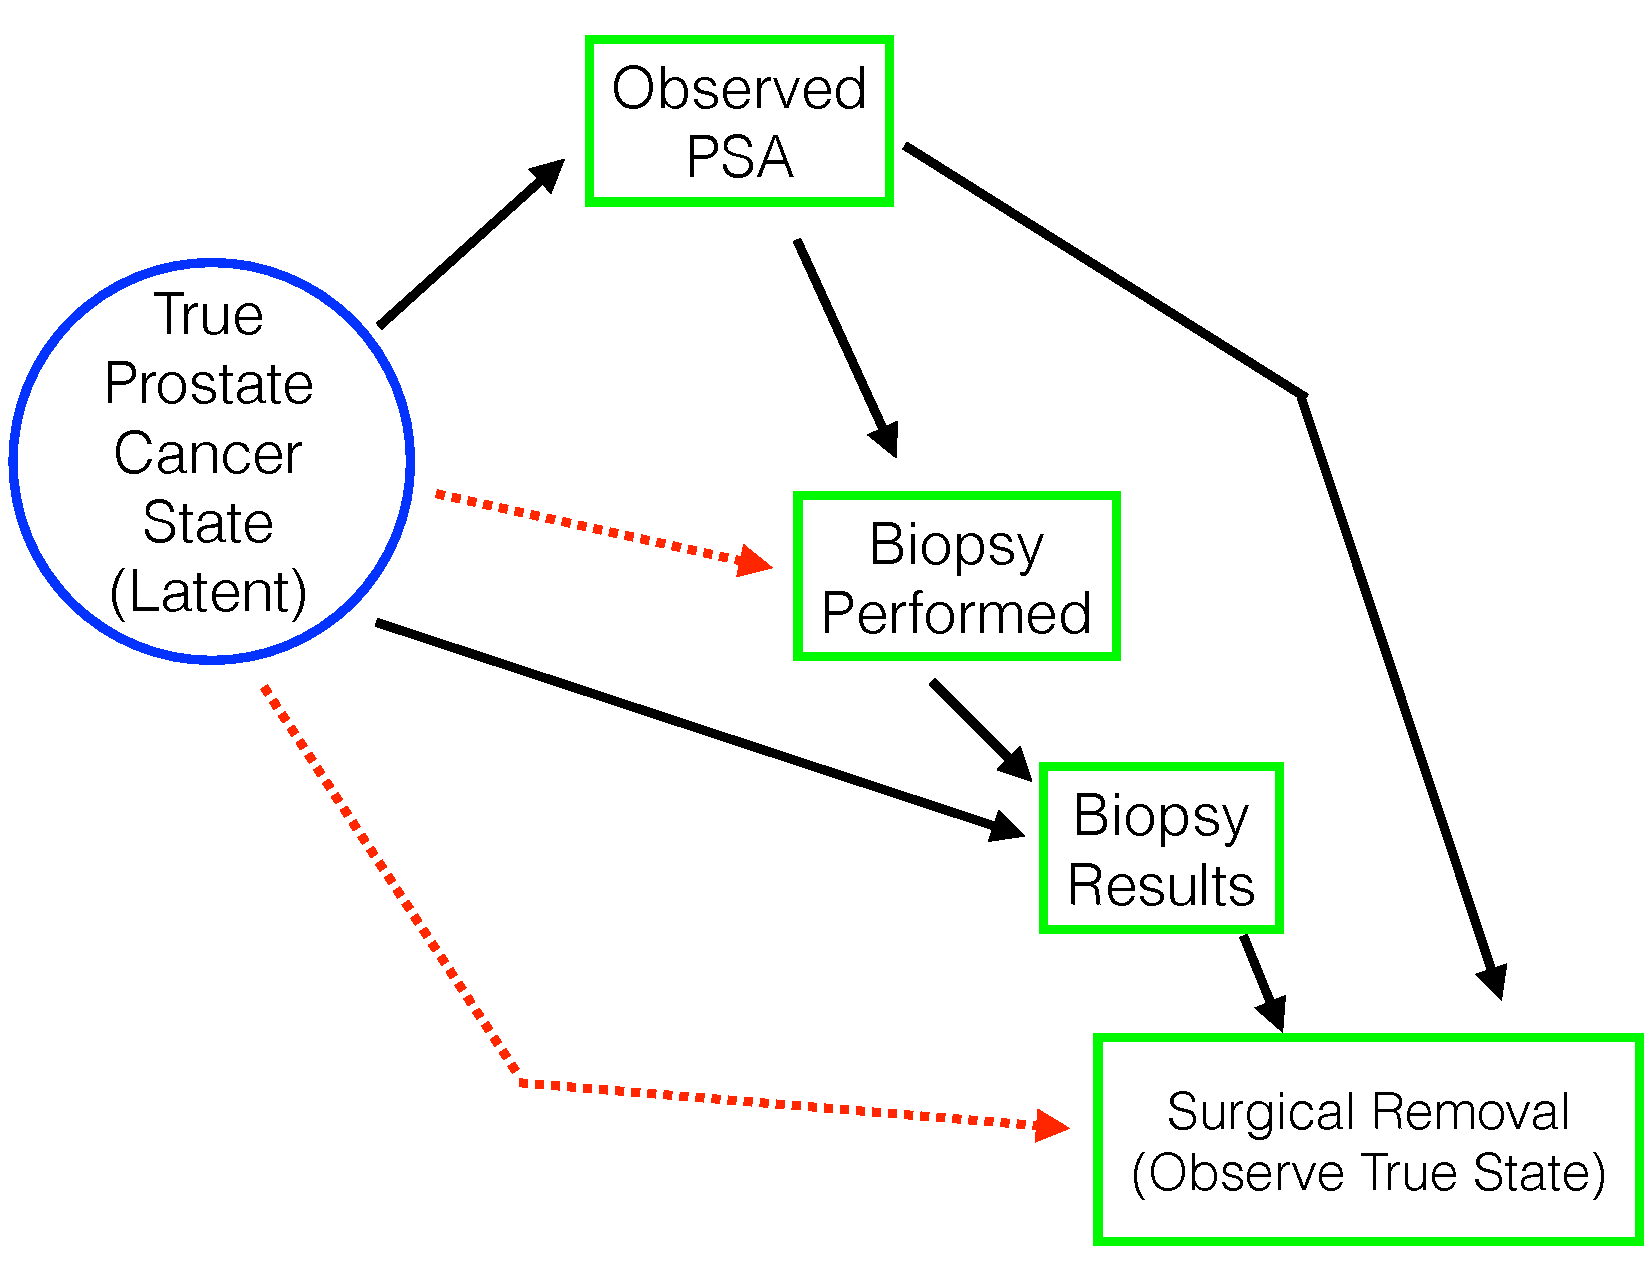
\includegraphics[width=\textwidth]{dag3}
\caption{}%Informative Observation Process}
\label{fig:dag3}
\end{subfigure}
\caption{DAGs describing the relationships between latent class (circled) and observed measurements (squared) (a) at a single point in time, (b) over time, and (c) in the presence of an informative observation process.}
\end{center}
\end{figure}

Our proposed model is similar to Lin et al. in 2002\nocite{Lin2002}, which first proposed a latent class approach to joint analysis of longitudinal PSA and time-to-diagnosis of prostate cancer, extending developments in joint models by Schluchter (1992)\nocite{Schluchter1992}, DeGruttola and Tu (1994)\nocite{DeGruttola1994}, and Henderson, Diggle, and Dobson (2000)\nocite{Henderson2000}. This joint latent class model (JLCM) has since been applied in many settings, including an extension of the method by Proust-Lima and Taylor (2009)\nocite{Proust2009} to develop a dynamic prognostic tool for prostate cancer recurrence after radiation therapy. Use of JLCM is motivated by interest in modeling differential risk and disease progression across a population and classifying individuals with similar outcomes, but, unlike our approach, typically does not involve a priori specification of classes of interest. 

In contrast to the model we are proposing, the JLCM model of Lin et al. assumes that prostate cancer diagnoses are both correct -- ignoring measurement error in diagnostic biopsies -- and a reflection of time of onset. On the contrary, diagnosis of low risk disease typically follows a physician's recommendation to perform a biopsy rather than presentation of clinical symptoms. To this point, the conditional independence assumption is suspect as observation of high PSA typically triggers biopsy recommendations. The same concern is present for predicting cancer state in an active surveillance population; biopsies are not always performed annually and, as a patient continues in the program, PSA kinetics are increasingly relied on for biopsy recommendations. The proposed model addresses this limitation by modeling reclassification with a pooled logistic regression model \cite{Cupples1988, D'Agostino1990} and modifying the conditional independence assumption to include conditioning on the presence of a biopsy. Moreover, under the assumption that the choice to get a biopsy depends on observed factors (PSA, patient characteristics and past biopsy results), i.e., that biopsy results are missing at random (MAR), unbiased identification of latent classes in a likelihood-based Bayesian framework does not require specification of a probability model for biopsy occurrence \cite{Little2014}. A similar line of reasoning can be followed for the decision to undergo surgical removal of the prostate, resulting in observation of the true cancer state. Under the MAR assumption, it is unnecessary to specify a model for the probability of electing surgery. 

We also offer a novel extension to the proposed model that allows for observation of biopsy results and the true cancer state to be missing not at random (MNAR). Consider the dotted lines in the DAG in Figure 1(c)-- if true cancer state is associated with the choice to perform a biopsy or undergo surgery after conditioning on observed PSA and biopsy results, then informative missingness is present and predictions will be biased \cite{Wu1988}. In response, we propose including cancer state as a predictor in regression models for the probability having a biopsy and having surgery at each annual interval. In this way, the dependence between observing the outcome and its value is accommodated.
This approach is similar to the latent class dropout model, proposed by Roy (2003, 2007)\nocite{Roy2003,Roy2007}, a type of shared parameter model \cite{Follmann1995} with discrete random effect. Unlike Roy's model for intermittent missingness which models latent class conditional on the observation process, we follow the model formulation outlined in Albert and Follmann (2009)\nocite{Albert2009}, specifying distributions for the outcome and the observation process conditional on cancer state.

Finally, in order to support decision-making in a clinical setting, we have developed an importance sampling algorithm to enable real-time updating of model predictions\cite{Geweke1989}. 


This paper is organized as follows. In Section 2, we describe data from an active surveillance cohort at Johns Hopkins. A joint hierarchical model for latent class prediction is outlined in Section 3, including a description of Bayesian estimation procedures. In Section 4, we propose and implement additions to the model in order to account for likely informativeness of biopsy and cancer state observations. Section 5 presents an application of the model to the active surveillance cohort. Then, importance sampling methods to obtain quick predictions update are detailed and demonstrated in Section 6. We close with a discussion.


\section{Active Surveillance Program for Prostate Cancer at Johns Hopkins}
As of Month Year, the Johns Hopkins Active Surveillance cohort has enrolled XX prostate cancer patients since 1995 (CITE). \textit{Still waiting for Mufaddal to send me this information so that we are consistent across papers.} In this study, patients with very-low-risk or low-risk prostate cancer diagnoses (according to criteria outlined in Epstein et al. (1994)\nocite{Epstein1994}, including biopsy Gleason score of 6) who elect to delay curative intervention in favor of active surveillance are followed prospectively. Characteristics of diagnostic biopsy and results of all prior PSA tests are collected at enrollment. As part of the surveillance regimen, PSA tests are typically performed every six months, and biopsies are performed annually, though these intervals vary; the results of all tests are recorded. Curative intervention is recommended upon biopsy reclassification, that is, when the Gleason score assigned to a biopsy exceeds 6. Some patients also choose to undergo curative intervention prior to reclassification. For patients who elect surgical removal of the prostate (whether prior to or after reclassification), Gleason score determination based on full pathologic analysis of the prostate specimen is also recorded.

\section{Joint Hierarchical Latent Class Model}

We have developed a Bayesian, joint hierarchical model to predict the underlying cancer state of patients enrolled in active surveillance. Predictions are made by incorporating information from repeated PSA and biopsy measurements for all individuals, as well as true cancer state information observed in a subset of the cohort. In this section, we first present notation before specifying models for each component of the likelihood (partially-observed latent class, PSA, and biopsy data) and defining the full likelihood. Next, we complete Bayesian specification of the model by defining the joint posterior distribution and discussing prior distributions for model parameters.  

\subsection{Notation} 
%\textit{This subsection may not be necessary.}
We first define each individual's underlying true cancer state, $\eta_i$, as either indolent, $\eta_i=0$, or aggressive, $\eta_i=1,$ for all cohort members $i=1,\dots,n$.  An individual's cancer state influences his observed PSA values, which we denote with $M_i$-length vector $\bmY_i$, as well as his biopsy results. Biopsy data is categorized into discrete, annual time intervals with $(B_{ij}, R_{ij})$ denoting binary variables that indicate whether a biopsy was performed and reclassification observed, respectively, for individual $i$ in year $j$.  Finally, $S_{ij}$ is an indicator of surgery for individual $i$ in year $j$. 
%(Further description cancer state is provided below.)
%(If no biopsy was performed, $B_{ij}=0$, then reclassification was not observed, $R_{ij}=0$.)
%These variables are recorded for all individuals until any curative intervention (including surgery), death, or loss-to-follow-up, defined as two years without any PSA or biopsy measurements.
%Details about follow-up and time interval partitioning could be moved to Application

\subsection{True Cancer State}
%The goal of analysis is to predict an individual's true cancer state, which we define using...
We first define each individual's true cancer state, $\eta_i$, using a dichotomized summary of the Gleason score that would be assigned if his entire prostate were to be removed and pathologic analysis performed:
\beas
\eta_i&=&
\left\{
\begin{array}{l l}
0 & \qquad \text{indolent; Gleason score for individual } i=6 \\
1 & \qquad \text{aggressive; Gleason score for individual } i \geq 7\\
\end{array} \right.
\eeas 
%make sure distinction between indolent and aggressive is laid out in intro and background
Since we observe this true cancer state on a subset of patients in active surveillance who choose surgical removal of the prostate, $\eta$ is best described, in the context of this model, as a partially observed latent variable. Cancer state is then modeled as a Bernoulli random variable, $\eta_i \sim Bern(\rho)$, where we assume a shared underlying probability of aggressive cancer, $\rho$, as our data do not include any baseline predictors of cancer state (other than PSA and biopsy measurements), such as genetic markers or family history.

This definition assumes that there is no variability in grading for full prostate specimens and that all observed grade determinations are correct. It also assumes that an individual's cancer categorization does not change over the time period under surveillance, i.e., that upgrading is due to sampling error at diagnosis rather than tumor dedifferentiation since diagnosis.  Under this conceptual framework, a prostate cancer is assumed to manifest its true state over time. More lethal cancers are considered fundamentally different from indolent ones from inception and it is assumed that, while tumor volume would likely differ, the same histologic category (i.e. Gleason $=6$ vs. Gleason $\geq7$) would be observed if a full pathologic analysis was performed earlier.  

\subsection{Longitudinal PSA Measurements}
Next, we specify a regression model for PSA, a time-varying biomarker dependent on an individual's true cancer state. PSA is also expected to increase with age and is independently influenced by additional factors including prostate volume and other sources of inflammation. We cannot observe an individual's true PSA; we only observe imprecise measurements of PSA at some points in time.

To reflect these characteristics, we use a mixed effects model to model the anticipated trajectory of an individual's PSA as they age \cite{Laird1982}. In this model, mean effects for predictors are allowed to vary across groups defined by partially latent class. Specifically, we expect the PSA of those with more aggressive cancer to have a higher level and steeper slope than those with indolent cancer (although we do not impose any restrictions on the model to enforce this expectation).  Random effects allow for individuals within each group to have intercepts and slopes that differ from the latent class means. We specify the following mixed effects model: 
\beas
\big[\, Y_{im} | \eta_i=k, \bmX_{im}, \bmZ_{im}\,\big] = \bmX_{im}\bmbeta + \bmZ_{im}\bmb_i + \epsilon_{im}
\eeas
where $Y_{im}$ is the observed (log-transformed) PSA and $\bmX_{im}$ and $\bmZ_{im}$ are vectors of covariates for individual $i$'s $m$th PSA measurement, $\bmbeta$ is a parameter vector for fixed effects, and $\bmb_i$ is the patient-specific vector of random effects. Following the specification of a Bayesian mixed effects model presented by Gelman and Hill (2006)\nocite{Gelman2006}, unscaled random effects are centered at the mean effects for each latent class $k$, $\bmmu_k$:
\beas
\big[\check{\bmb_i} | \eta_i=k\big] \sim MVN ( \bmmu_k, \Sigma_k), \quad k=0,1 
\eeas
where $\Sigma_k$ is a covariance matrix that allows for correlation between random effects. Random effects are then scaled with parameter vector $\bmxi$: $\bmb_i = diag(\check{\bmb_i}\bmxi^T)$.

Lastly, residuals $\epsilon_{im}$ are assumed to follow a normal distribution with mean 0 and variance $\sigma^2$. As a result, the vector of observed PSAs for individual $i$, $\bmY_i=(Y_{i1},\mydots,Y_{iM_i})$, follows a multivariate normal distribution. 

%Here, we assume that the covariance matrix is the same across classes. This assumption aids model identifiability and convergence by reducing the number of parameters to be estimated and was made only after examining the covariance estimates obtained by fitting the mixed effects models in the subset of patients with latent class observed and confirming its plausibility.  

%Explain what covariates are in X and Z in application section

\subsection{Repeated Biopsy Outcomes}
Finally, we consider the likelihood contribution for biopsy results. An individual's true prostate cancer state also influences, but does not determine, the findings of biopsies performed as a part of the active surveillance regimen. While biopsies target areas of the prostate where tumors are expected to be located, as identified by pre-biopsy ultrasound or MRI, biopsied tissue constitutes only a sample of the prostate. (For example, the volume of tissue collected in a typical 12-core biopsy only includes, at most, 0.5$\%$ of the total prostate volume,)  Moreover, sectioning of biopsied tissues for evaluation can introduce further uncertainty into histologic assessment, and overgrading is possible. As a result, biopsy-determined Gleason scores have imperfect sensitivity and specificity for predicting true cancer state.  

%We model reclassification, i.e., determination for Gleason 7 or higher, for all biopsies performed.
%Since the frequency and timing of biopsies varies across patients, we categorize biopsy times into annual intervals where time is measured since diagnosis. 
Since the frequency of biopsies are typically dictated by AS protocol, we categorize biopsy times and results into discrete time intervals. If individual $i$ has a biopsy during interval $j$, it is indicated by $B_{ij}=1$. Then, we define $R_{ij}$ as a binary outcome denoting reclassification during this interval. If a biopsy is performed, we use a logistic regression model to predict the probability of grade reclassification within that interval conditional on true cancer state and time-varying patient characteristics:
\bea
\label{eq:p_rc}
P(R_{ij}=1 | \eta_i=k, \bmV_{ij}, \bmgamma) = \text{logit}^{-1}\big( \bmV_{ij}(k)\bmgamma \big)
\eea
where $\bmV_{ij}(k)$, is a matrix of time-varying predictors including cancer state $\eta_i=k$ and $\bmgamma$ is a parameter vector. If a biopsy is not performed, $B_{ij}=0$, then reclassification cannot be observed and $R_{ij}$ is undefined. 

Using this logistic regression model within each interval where a biopsy is performed, we model time-until-reclassification using a pooled logistic regression model, that is, we take the product of the probability of the observed result over all biopsies performed \cite{D'Agostino1990}. Intervals without biopsies do not contribute to this product, and $B_{ij}$ is only defined for intervals up to the time of reclassification or censoring, $j=1,\dots,J_i$.

%Note, $B_{ij}$ is only defined for intervals prior to reclassification, that is for $j=1,\dots,J_i$ where $J_i$ is the time of reclassification or final interval under observation for individual $i$.


%Under the assumption of no unobserved confounders between the choice to perform a biopsy and the results, only intervals with a biopsy contribute to the likelihood. (We consider this assumption in more detail in Section 4.)

%If no biopsy is performed, $B_{ij}=0$, then reclassification cannot be observed, i.e. $P(R_{ij}=1|\eta_i=k, \bmV_{ij},B _{ij}=0, \bmgamma) = 0$. 
%deal with possibility of multiple biopsies in Sec 5
%give the length of our intervals in section 5

%

\subsection{Likelihood}
%\subsection{Model Estimation}

The likelihood for the proposed model can be written as:
\bea
&&L\Big(\rho, \bmbeta, (\bmmu_k, \Sigma_k), k=0,1, \bmgamma, (\eta_i, \bmb_i)  \, | \,\big( \bmY_i, \underline{\bmX_i}, \underline{\bmZ_i}, (B_{ij}, R_{ij}, \bmV_{ij}), j=1,\mydots,J_i \big), i=1,\mydots,n \Big) \nonumber \\
&& \quad =  \prod_{i=1}^{n}  \,  \rho^{\eta_i}\,(1-\rho)^{1-\eta_i}\, f(\bmY_i | \eta_i, \underline{\bmX_i}, \underline{\bmZ_i}, \bmb_i, \bmbeta, \sigma^2) \, g(\bmb_i |  \bmmu_{\eta_i}, \Sigma_{\eta_i})  \nonumber \\
\label{eq:lik-unadj}
&& \qquad \qquad \prod_{j=1}^{J_i}  \big(P(R_{ij}=1 | \eta_i, \bmV_{ij}, \bmgamma) ^{R_{ij}} P(R_{ij}=0 | \eta_i, \bmV_{ij}, \bmgamma)^{1-R_{ij}} \big)^{B_{ij}}
\eea
where $f$ and $g$ are multivariate normal densities for the vector of log-transformed PSAs, $\bmY_i$, and random effects $\bmb_i$, respectively, for individual $i$, each with mean and covariance as defined above, given covariance matrices $\underline{\bmX_i} = [X_{i1},\dots, X_{iM_i}]$ and $\underline{\bmZ_i} = [Z_{i1},\dots,Z_{iM_i}]$. 

We note that dependence structures codified in the Figure 1 (a) and (b) DAGs are reflected in this likelihood. First, PSA measurements, $\bmY_i$, are independent of biopsy results conditional on true cancer state. Second, biopsy results are also conditionally independent given true cancer state. 

\subsection{Bayesian Estimation}

We use a Bayesian approach to estimate the proposed joint latent class model. Standard prior distributions are available for model parameters including, for example a beta prior on the probability of having aggressive cancer ($\eta=1$) and normal priors on logistic regression model coefficients. Prior specification for the mixed effects model can follow the Bayesian estimation procedure outlined in Gelman and Hill (2006) for a linear mixed effects model with correlated random effects using a scaled inverse Wishart prior\nocite{Gelman2006}. %Alternatively, an inverse prior could be used for the covariance matrix \cite{Gelfand1995}, keeping in mind known limitations \cite{Kass2006}.

After specifying priors for all model parameters, the joint posterior distribution of the parameters and partially-latent classes is given by:
%\begin{small}
\beas
&& p\Big(\rho, \bmbeta, (\bmmu_k,\Sigma_k), \bmgamma, (\eta_i,\bmb_i) \,| \, \big( \bmY_i, \underline{\bmX_i}, \underline{\bmZ_i}, (B_{ij}, R_{ij}, \bmV_{ij}) \big); \bmTheta\Big) \\
&&\qquad  \propto L\Big(\rho,  \bmbeta, (\bmmu_k, \Sigma_k), \bmgamma, (\eta_i, \bmb_i)  \, | \,\big(\bmY_i, \underline{\bmX_i}, \underline{\bmZ_i}, (B_{ij}, R_{ij}, \bmV_{ij})\big) \Big) \times \bmpi(\rho,\bmbeta, (\bmmu_k, \Sigma_k), \bmgamma |\bmTheta)
\eeas
%\end{small}
where $\bmpi(\cdot | \bmTheta)$ denotes the joint prior density for model parameters with hyper priors $\bmTheta$ and indexing $k=0,1$, $j=1,\mydots,J_i,$ and $i=1,\mydots,n$. 



\section{Informative Observation Process}
In this section, we propose an addition to the joint latent class model presented above in order to account for informative missingness. 

The model outlined in Section 3 assumes that unobserved biopsy results, i.e. $R_{ij}$ for intervals where $B_{ij}=0$, and true cancer state are either missing completely at random (MCAR) or missing at random (MAR) \cite{Little2014}. The likelihood given in (\ref{eq:lik-unadj}) is consistent with both scenarios: if observations are MCAR, no modeling of the missingness mechanism is necessary and, if observations are MAR, the missingness mechanism is known and can be explicity modeled. In the latter case, terms modeling the probability of observing true cancer state or biopsy results are not needed in the likelihood for our Bayesian approach because they do not contain parameters needed for prediction and thus fall out when parsing the joint posterior into full conditional posteriors for parameters of interest.

The likelihood in (\ref{eq:lik-unadj}) is not consistent, however, with the possibility that the true cancer state influences whether an individual has a biopsy or surgery performed (the latter resulting in observation of the cancer state) or, said another way, that the observation process itself is informative of true cancer state. This scenario is an example of observations missing not at random (MNAR) and is depicted in Figure 1(c). If missingness is indeed informative, the arrows pointing from cancer state to biopsy performance and surgical removal of the prostate and present and the model given in Section 3 will result in biased prediction of the true cancer state. 

To allow for the possibility of an informative observation process (IOP), we propose explicitly modeling the presence of biopsies and surgery as dependent on the true cancer state. This approach could be described as a shared parameter model with a discrete random effect where the prediction and interpretation of the random effect is of interest \cite{Follmann1995}. 

First, we specify a model for the probability that patient $i$ receives a biopsy in each time interval $j$ conditional on latent class, $\eta_i$, and time-varying covariates, $\bmU_{ij}(k)$:  
\bea
\label{eq:p_bx}
P(B_{ij}=1 | \eta_i=k, \bmU_{ij}, \bmnu) = \text{logit}^{-1}\big( \bmU_{ij}(k) \bmnu \big)
\eea
where $\bmnu$ is a parameter vector. Individual $i$ contributes $P(B_{ij}=1 | \eta_i=k, \bmU_{ij}, \bmnu)^{B_{ij}}P(B_{ij}=0 | \eta_i=k, \bmU_{ij}, \bmnu)^{1-B_{ij}}$ to the likelihood for every time interval up until reclassification or censoring.

Next, we define $S_{ij}$, an indicator of surgical removal of the prostate for individual $i$ during time $j$ and model the time-to-surgery using a pooled logistic regression model with the probability of surgery in each time interval defined as:
\beas
P(S_{ij}=1 | \eta_i=k, \bmW_{ij}, \bmomega) = \text{logit}^{-1}\big( \bmW_{ij}(k)\bmomega \big)
\eeas
where $\bmW_{ij}$ is a matrix of time-varying predictors including cancer state $\eta_i=k$ and $\bmomega$ is a parameter vector. The possibility of surgery extends beyond the time of reclassification as the decision to undergo prostatectomy is often informed by biopsy results. Accordingly, $S_{ij}$ is defined for all time intervals for which a patient is under observation, which may continue past reclassification. We denote the final interval under observation as $J_{S_i}$ for individual $i$.

For both IOP models, time-varying covariates ($U_{ij}$ and $W_{ij}$) may include information from past intervals, including the number and results of past biopsies, which would likely influence future biopsy and surgery decisions.


Finally, the likelihood and joint posterior for the proposed model can be updated to include the IOP models:
\bea
&&L\Big(\rho, \bmbeta, (\bmmu_k, \Sigma_k), \bmnu, \bmgamma, \bmomega, (\eta_i, \bmb_i)  \, | \,\big( \bmY_i, \underline{\bmX_i}, \underline{\bmZ_i}, (B_{ij}, \bmU_{ij}), (R_{ij}, \bmV_{ij}), (S_{ij}, \bmW_{ij}) \big), i=1,\mydots,n \Big) \nonumber \\
&& \quad =  \prod_{i=1}^{n}  \,  \rho^{\eta_i}\,(1-\rho)^{1-\eta_i}\, f(\bmY_i | \eta_i, \underline{\bmX_i}, \underline{\bmZ_i}, \bmb_i, \bmbeta, \sigma^2) \, g(\bmb_i |  \bmmu_{\eta_i}, \Sigma_{\eta_i})  \nonumber \\
&& \qquad \qquad \prod_{j=1}^{J_i}  P(B_{ij}=1 | \eta_i, \bmU_{ij}, \bmnu) ^{B_{ij}} P(B_{ij}=0 | \eta_i, \bmU_{ij}, \bmnu)^{1-B_{ij}}  \nonumber \\
&& \qquad \qquad \qquad  \qquad \big(P(R_{ij}=1 | \eta_i, \bmV_{ij}, \bmgamma) ^{R_{ij}} P(R_{ij}=0 | \eta_i, \bmV_{ij}, \bmgamma)^{1-R_{ij}} \big)^{B_{ij}} \nonumber \\
\label{eq:lik-inf}
&& \qquad \qquad  \prod_{j=1}^{J_{S_i}}  P(S_{ij}=1 | \eta_i, \bmW_{ij}, \bmomega) ^{S_{ij}} P(S_{ij}=0 | \eta_i, \bmW_{ij}, \bmomega)^{1-S_{ij}} .
\eea
and 
\bea
&& p\Big(\rho, \bmbeta, (\bmmu_k,\Sigma_k), \bmnu, \bmgamma, \bmomega, (\eta_i,\bmb_i) \,| \, \big( \bmY_i, \underline{\bmX_i}, \underline{\bmZ_i}, (B_{ij}, \bmU_{ij}), (R_{ij}, \bmV_{ij}), (S_{ij}, \bmW_{ij}) \big); \bmTheta\Big) \nonumber\\
&&\qquad  \propto L\Big(\rho,  \bmbeta, (\bmmu_k, \Sigma_k), \bmnu, \bmgamma, \bmomega, (\eta_i, \bmb_i)  \, | \,\big(\bmY_i, \underline{\bmX_i}, \underline{\bmZ_i},(B_{ij}, \bmU_{ij}), (R_{ij}, \bmV_{ij}), (S_{ij}, \bmW_{ij})\big) \Big)\nonumber\\
\label{eq:post-inf}
&& \qquad \qquad \qquad \times \bmpi\big(\rho,\bmbeta, (\bmmu_k, \Sigma_k), \bmnu, \bmgamma, \bmomega |\bmTheta\big).
\eea


\section{Application}
\subsection{Methods}
We applied both the unadjusted and the IOP model to data from the Johns Hopkins Active Surveillance Cohort. Patients who met Epstein et al. (1994) criteria for ``very low risk", had at least two PSA measurements, and at least one post-diagnosis biopsy as of October 2014 were included in the analysis. Patients still active in the program were censored at this date. Otherwise, observations on a patient were censored when he received curative intervention (including radical prostatectomy, radiation therapy, hormone therapy, or cryotherapy), died, or was lost to follow-up. Loss to follow-up was defined as two years without a PSA  or biopsy after the last observation. 

PSA trajectory was modeled with a linear mixed effects model, as described in Section 3.3. Random effects for intercept and age ($\bmZ$), centered at the mean intercept and slope for each partially-latent class, were estimated for each patient in addition to fixed effects for prostate volume ($\bmX$). A shared covariance matrix was assumed for the random effects, i.e. $\Sigma_0=\Sigma_1,$ in order to aid identifiability. The plausibility of this assumption was confirmed by fitting the mixed effects model in the subset of patients with cancer state observed. 

Biopsy, reclassification, and surgery observations were categorized into annual intervals, since Johns Hopkins' active surveillance protocol is to perform a biopsy every year. A small number of intervals contained two biopsies (approximately 1$\%$). To accommodate this, we redefine the logistic regression model in Equation (\ref{eq:p_bx}) as the probability of any biopsies during the year. (We also considered modeling the number of biopsies with a Poisson regression model, but this approach did not improve model fit or predictive accuracy.) Also, for intervals with two biopsies, both contributed separately to the pooled logistic regression model for time-to-reclassification. 

In addition to cancer state, age, time since diagnosis, and calendar time were included as predictors in all logistic regression models. The number of previous biopsies was also included as a predictor in the biopsy and surgery submodels. The surgery submodel also included reclassification as well as other biopsy results (number of positive cores, maximum percent involvement of any core). Natural spline representations of predictors were used in place of linear representations when doing so improved model fit.

Model parameters and non-informative priors for the analysis are included in the model summary given in Figure \ref{fig:model-summary}. Posterior sampling was performed in \texttt{R2JAGS} with code available at \texttt{http://github.com/rycoley/XXX}. Simulated data (based on model estimates) is also provided.

Predictive accuracy was assessed in the following ways. First, the out-of-sample area-under-the-curve (AUC) and receiver operating characteristics (ROC) of posterior cancer state predictions were calculated among those participants for whom true state had been observed \cite{Hosmer2013}. AUC and ROC were found for both the unadjusted model (as described in Section 3) and the model adjusted for a possibly informative observation process (IOP). Second, calibration plots were drawn and examined in order to compare the posterior probability of biopsies, reclassification, and surgery in each person-year to the observed rates of these outcomes via natural spline regression.


\begin{figure}
\begin{center}
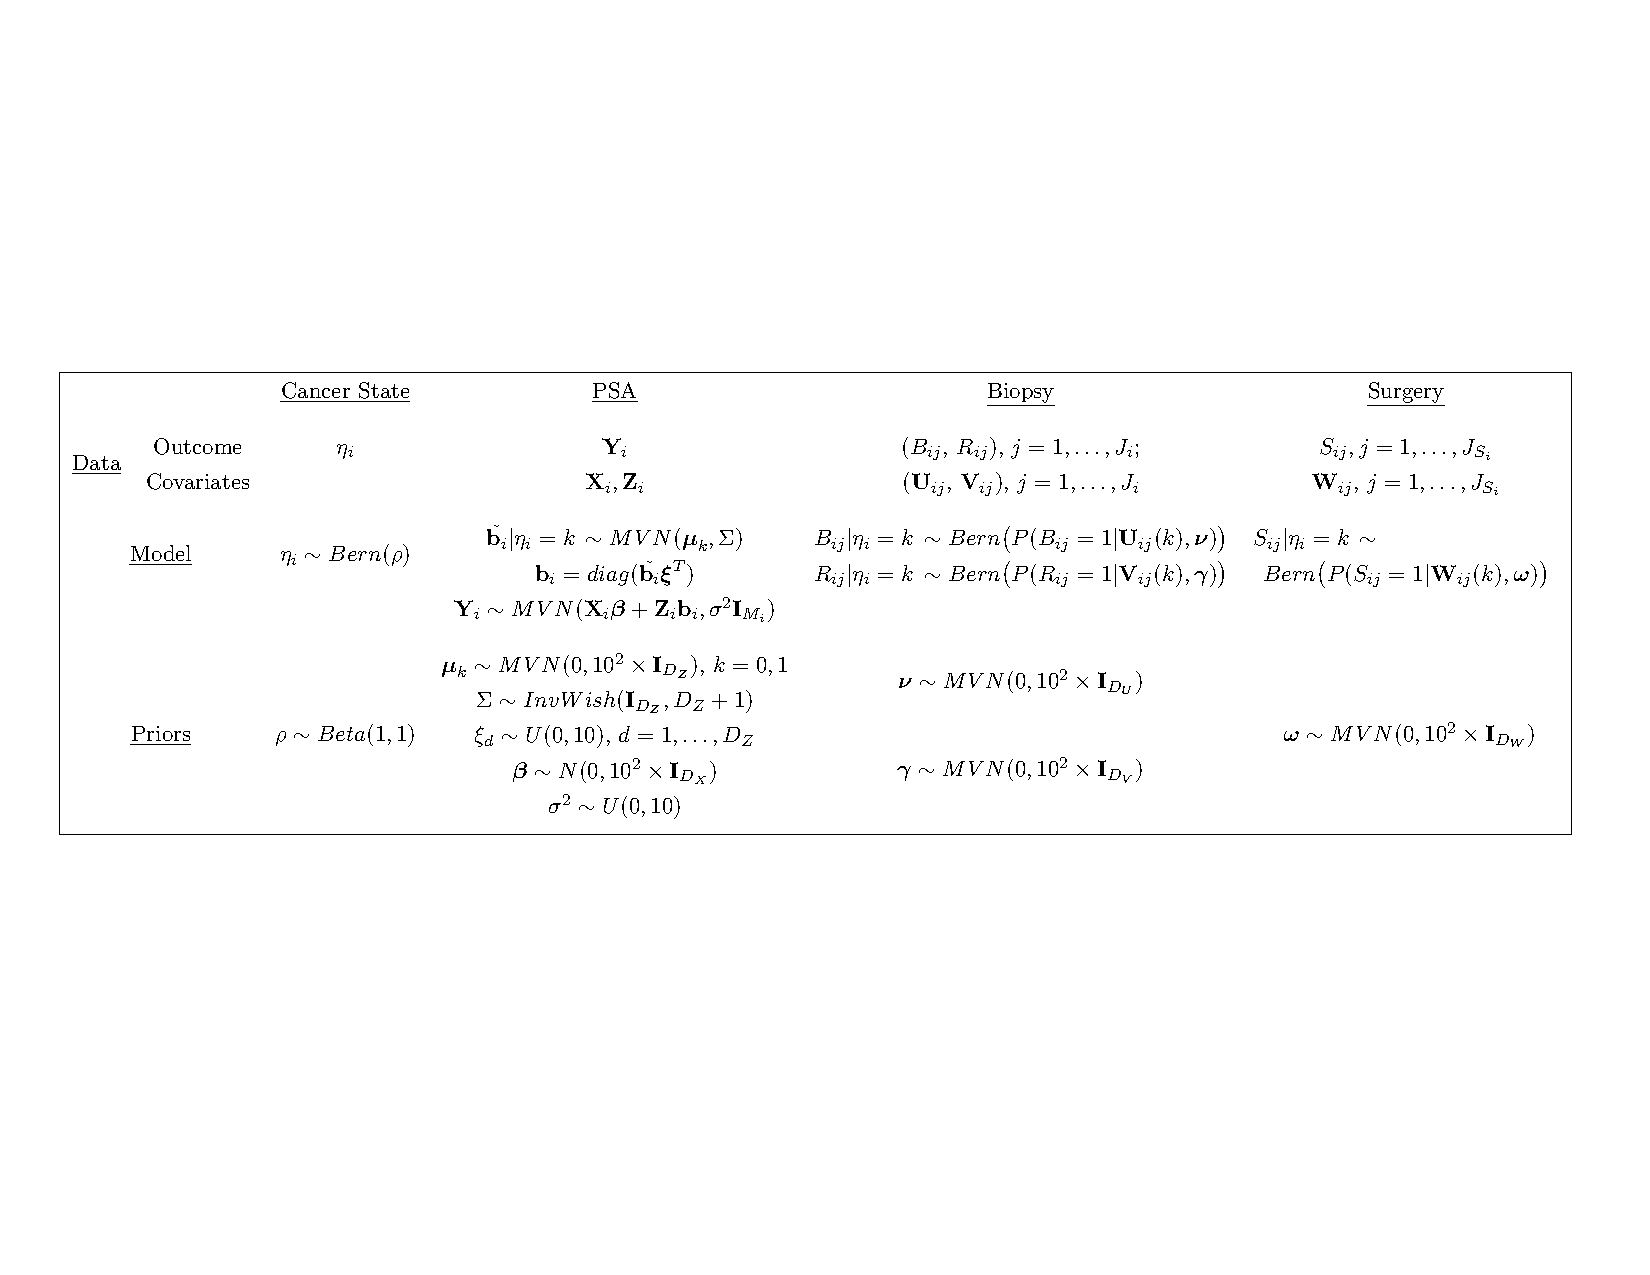
\includegraphics[width=\textwidth]{model-summary-table.pdf}
\caption{Model Summary. $D_X$ is the length of vector $\bmX$ and $\bmI_{D_X}$ is the identity matrix with dimension $D_X$.}
\label{fig:model-summary}
\end{center}
\end{figure}



\subsection{Results}
874 patients from the Johns Hopkins Active Surveillance cohort met the criteria for inclusion in this analysis. The number of observations and years of follow-up available for analysis are summarized in Table \ref{tab:num_obs}. Among the 874 patients included in the analysis, reclassification was observed in 160 patients (18$\%$). 167 patients (19$\%$) elected for surgical removal of the prostate (78 after experiencing reclassification), of which 161 had post-surgery full prostate Gleason score determination available. Results of post-surgery pathologic analysis in comparison to pre-surgery reclassification are given in Table \ref{tab:eta-vs-rc}. A total of 318 patients (36$\%$) were censored due to receiving some curative intervention, 130 (15$\%$) were lost to follow-up, and nineteen (2.2$\%$) were censored due to death. (No patients died of prostate cancer.) 407 patients (47$\%$) remained active in the program at the time of data collection for this analysis. 


\begin{table}
\begin{center}
\begin{tabular}{|c|c|c|}
\hline
 & Total $\#$ observations & Median $\#$ per patient (IQR) \\[5pt]
\hline
PSA & 10,425 & 10 (6,16)\\[5pt]
Biopsy & 2,741 & 3 (1,4)\\[5pt]
Years of follow-up & \multirow{2}{*}{4,980} & \multirow{2}{*}{5 (3,8)}\\
(prior to reclassification) & & \\[5pt]
\hline
\end{tabular}
\caption{Summary of observations and follow-up time for $n$=874 patients included in analysis.}
\label{tab:num_obs}
\end{center}
\end{table}

\begin{table}
\begin{center}
\begin{tabular}{|c|c|c|c|}
\hline
& \multicolumn{2}{|c|}{Reclassification} & \\
 & $R$=0 & $R$=1 & Total\\[5pt]
 \hline
Indolent, $\eta=0$ & 66  (69$\%$) & 17 (26$\%$) & 83 \\[5pt]
Aggressive, $\eta=1$ & 30 (31$\%$) & 48 (74$\%$) & 78\\[5pt]
 \hline 
 Total & 96 & 65 & 161\\[5pt]
\hline
\end{tabular}
\caption{Summary of post-surgery cancer state determination ($\eta$) compared to reclassification ($R$) on final biopsy with column percentages in subset of patients with true state observed ($n=161$)}
\label{tab:eta-vs-rc}
\end{center}
\end{table}


Figure \ref{fig:singles} shows the PSA and biopsy data available on a dozen patients in the cohort.  Plotting circles represent observed PSA values, with the scale given on the lefthand y-axis. Triangles represent biopsies, with open triangles indicating no biopsy in an annual interval (and, thus, no reclassification observed) and filled triangles indicating biopsy results; triangles at the bottom of the plot represent no grade reclassification while those at the top represent a Gleason score of 7 or higher on biopsy. Alongside the observed data, Figure \ref{fig:singles} also gives posterior predictions from the proposed model about each patient's true cancer state (above each plot), likely PSA trajectory, and risk of reclassification on a future biopsy (with scale given on righthand y-axis). Shaded credible intervals indicate the posterior distribution for these predictions with the darkest shading occurring at the posterior median. Note that no reclassification projections are given for those patients with grade reclassification observed, as they will not continue with biopsies.  

\begin{figure}
\begin{center}
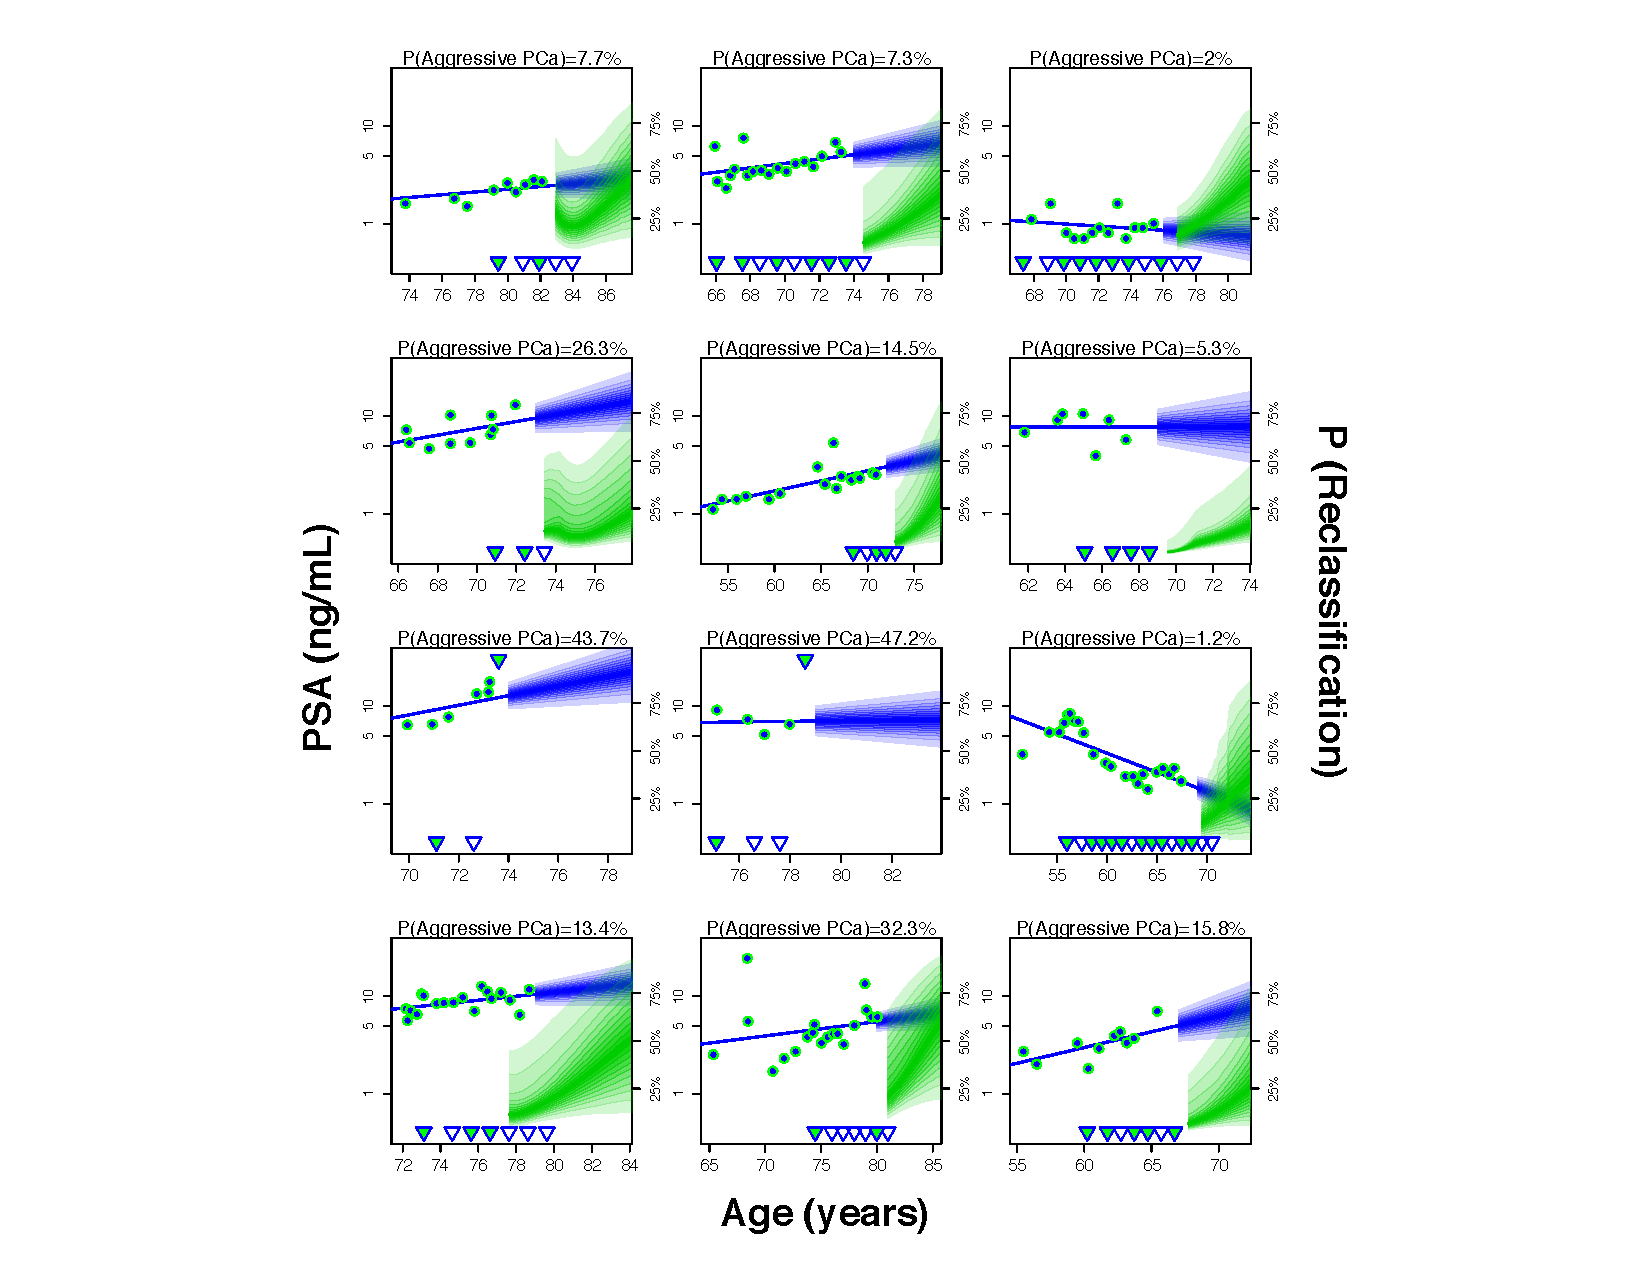
\includegraphics[width=\textwidth]{data-and-predictions.pdf}
\caption{PSA (circles) and reclassification (triangle) data for a dozen patients. Posterior probabilities of having aggressive prostate cancer are above each patient's data. Shaded intervals show posterior credible intervals around projected PSA (blue) and reclassification (green) trajectories. }
\label{fig:singles}
\end{center}
\end{figure}


The ROC curves and calibration plot in Figure \ref{fig:eta-accuracy} illustrate the proposed informative observation process (IOP) model's ability to accurately predict an individual's cancer state. The out-of-sample AUC among patients with true cancer state known is 0.75.  We also see that the IOP model outperforms the unadjusted model, which has an AUC of 0.72. In the right-hand panel, the calibration plot shows that posterior predictions of underlying aggressive cancer generally follow the observed rates (i.e., track the x=y axis), with the exception of very low risk predictions, where less data is available. In this plot, hashmarks at y=0 and y=1 show the observed cancer state for individuals against their posterior prediction on the x-axis. 
\begin{figure}
\begin{center}
\begin{subfigure}[b]{0.45\textwidth}
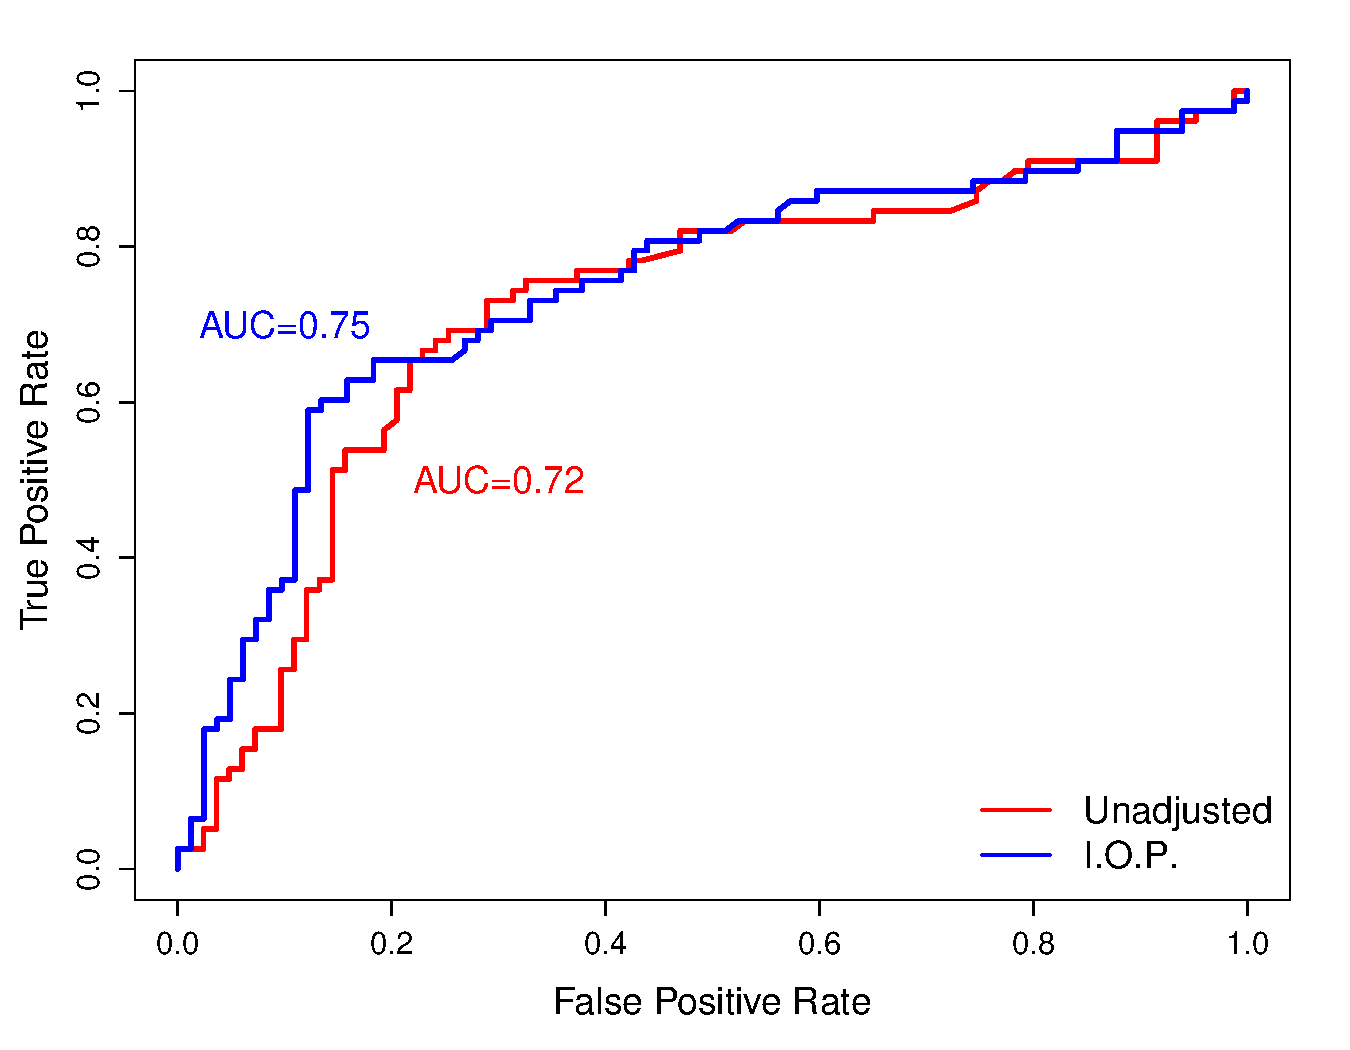
\includegraphics[width=\textwidth]{pred-vs-obs-eta-roc}
%\caption{}
\label{fig:roc}
\end{subfigure}
\begin{subfigure}[b]{0.45\textwidth}
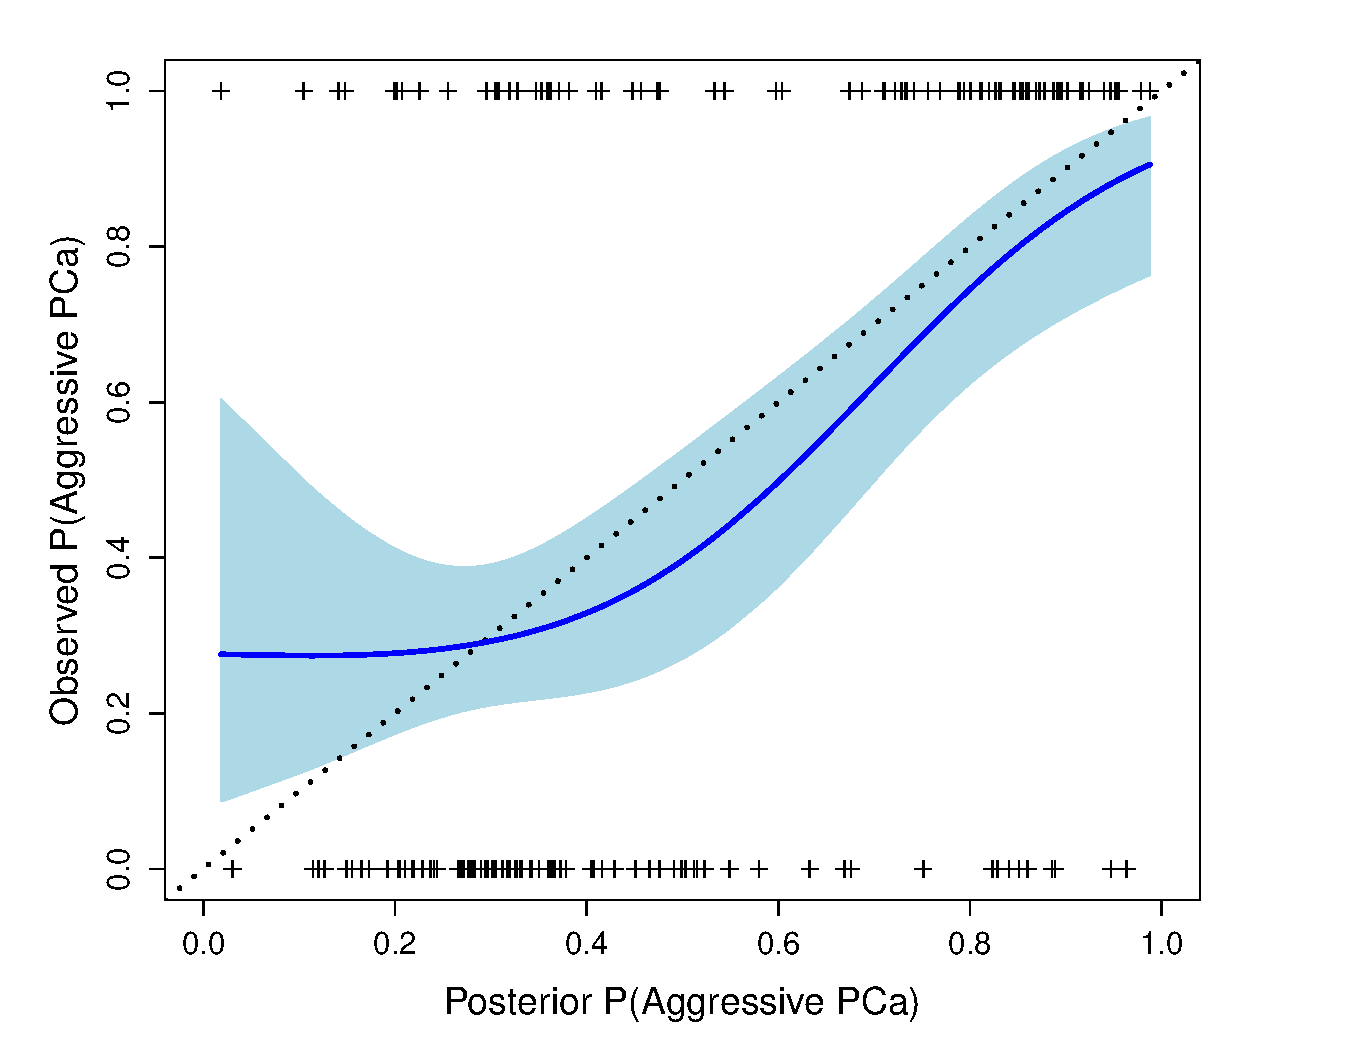
\includegraphics[width=\textwidth]{pred-vs-obs-eta}
%\caption{}
\label{fig:calibrartion-eta}
\end{subfigure}
\caption{ROC curve (left panel) and calibration plot (right panel) for predictions of underlying cancer state, $\eta$, among those with true state observed}
\label{fig:eta-accuracy}
\end{center}
\end{figure}

Posterior estimates from the mixed effects model for PSA are displayed in Figure \ref{fig:lme}. In this plot, each plotting circle represents the scaled random intercept (x-axis) and slope (y-axis) estimates for a single patient. Filled circles represent patients for whom the true cancer state was observed, with red indicating potentially lethal cancer found after surgery and green indicating a determination of indolent cancer. The color of open circles reflects the posterior probability of aggressive cancer, ranging from low (green) to high (red), among patients for whom true state was not observed. Finally, credible ellipses show the posterior mean and covariance of random effects for individuals in each partially latent class. We see that there is a fair amount of overlap in these intervals, indicating that PSA level and trajectory does not provide information about the true state for most patients. PSA  is more informative, however, for patients with particularly high or low levels and trajectories. 

\begin{figure}
\begin{center}
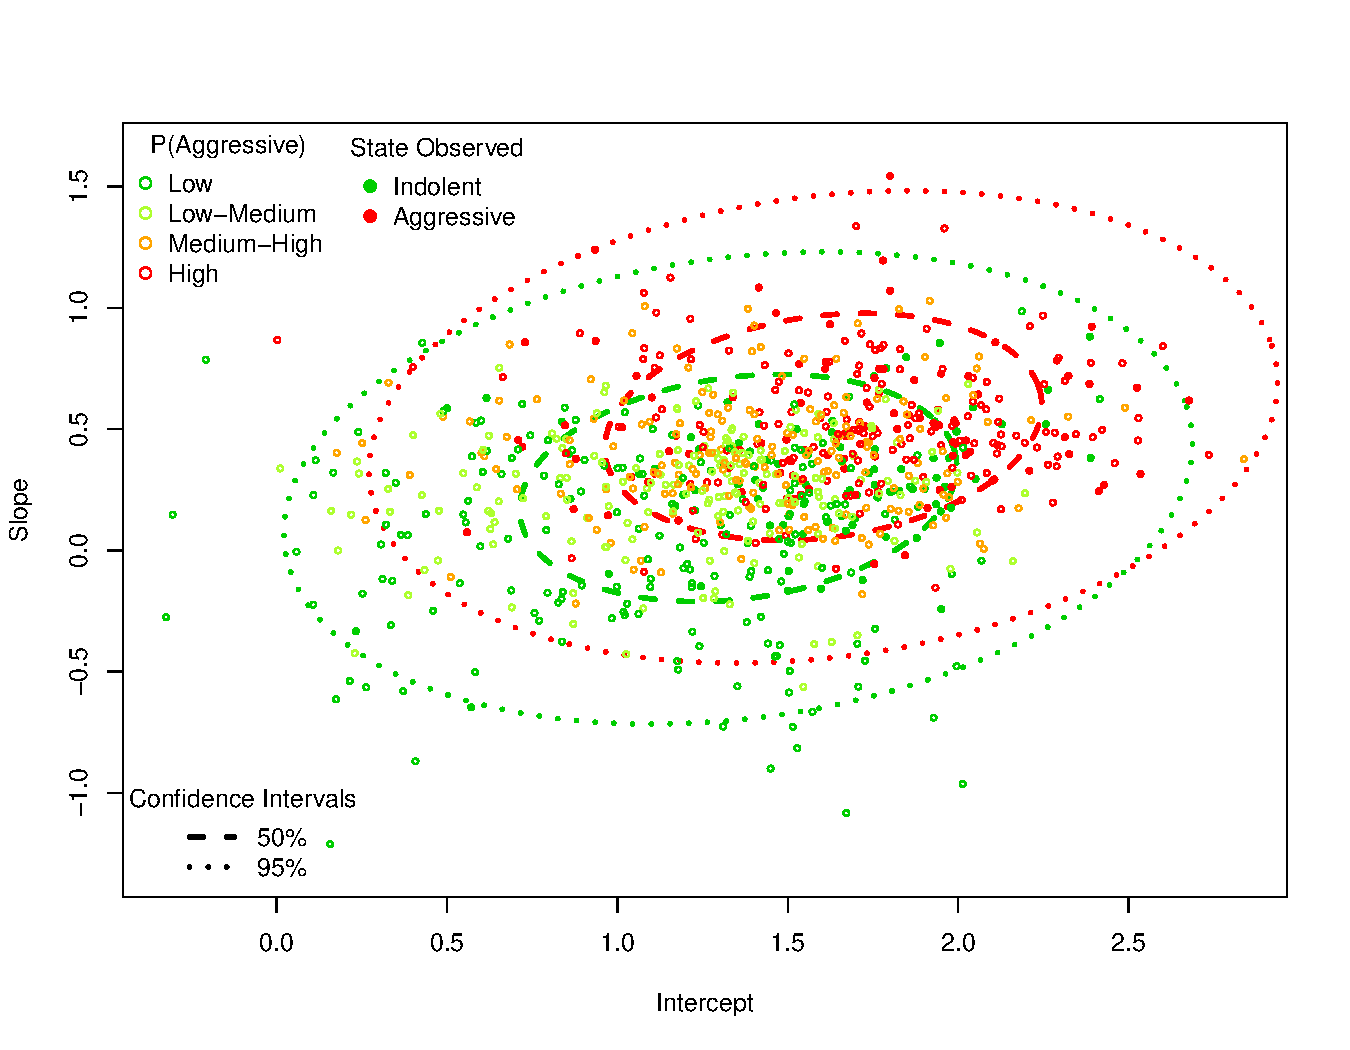
\includegraphics[width=0.8\textwidth]{random-effect-est.pdf}
\caption{Random effects estimates from stratified mixed effects model for PSA.}
\label{fig:lme}
\end{center}
\end{figure}

Calibration plots for posterior predictions of biopsy, reclassification, and surgery are given in Figure \ref{fig:calibration-all-bx}. Overall, posterior probabilities reflect observed rates of each outcome, especially in ranges with more data. Posterior predictions appear less accurate for reclassification but we note that the vast majority of person-years (87$\%$) have a predicted risk of reclassification below 10$\%$, where the model fits well. We suspect that the lack of strong predictors of reclassification limited our ability to accurately predict risk at higher ranges. (Only age, secular time, and time since diagnosis were available for inclusion in the reclassification model).

\begin{figure}
\begin{center}
\begin{subfigure}[b]{0.5\textwidth}
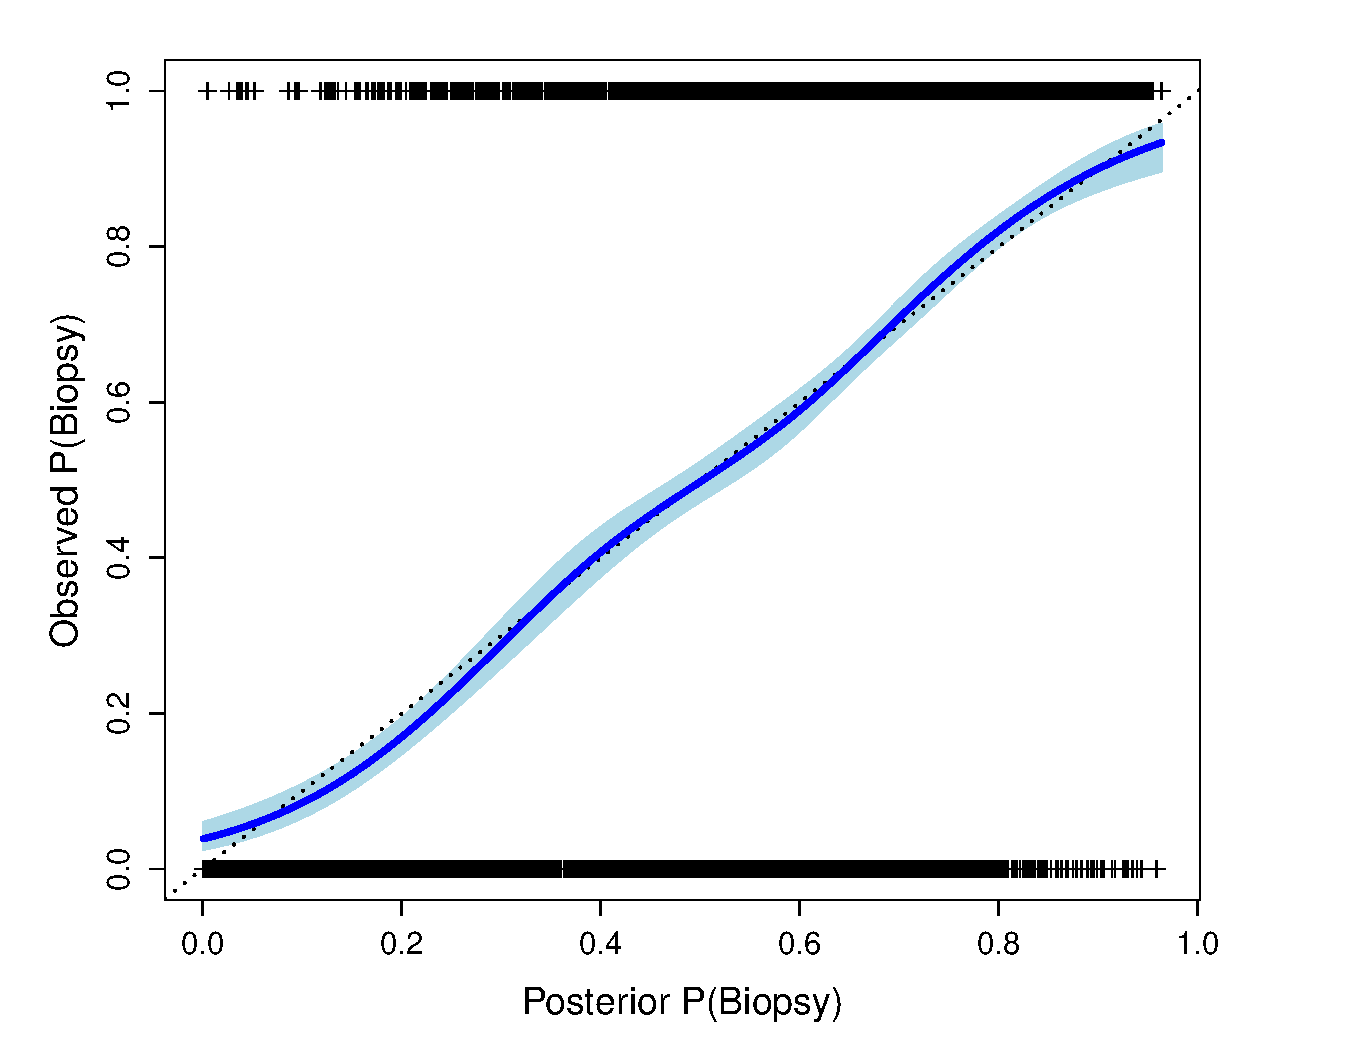
\includegraphics[width=\textwidth]{pred-vs-obs-bx.pdf}
%\caption{}
%\label{fig:calibration-bx}
\end{subfigure}
\begin{subfigure}[b]{0.5\textwidth}
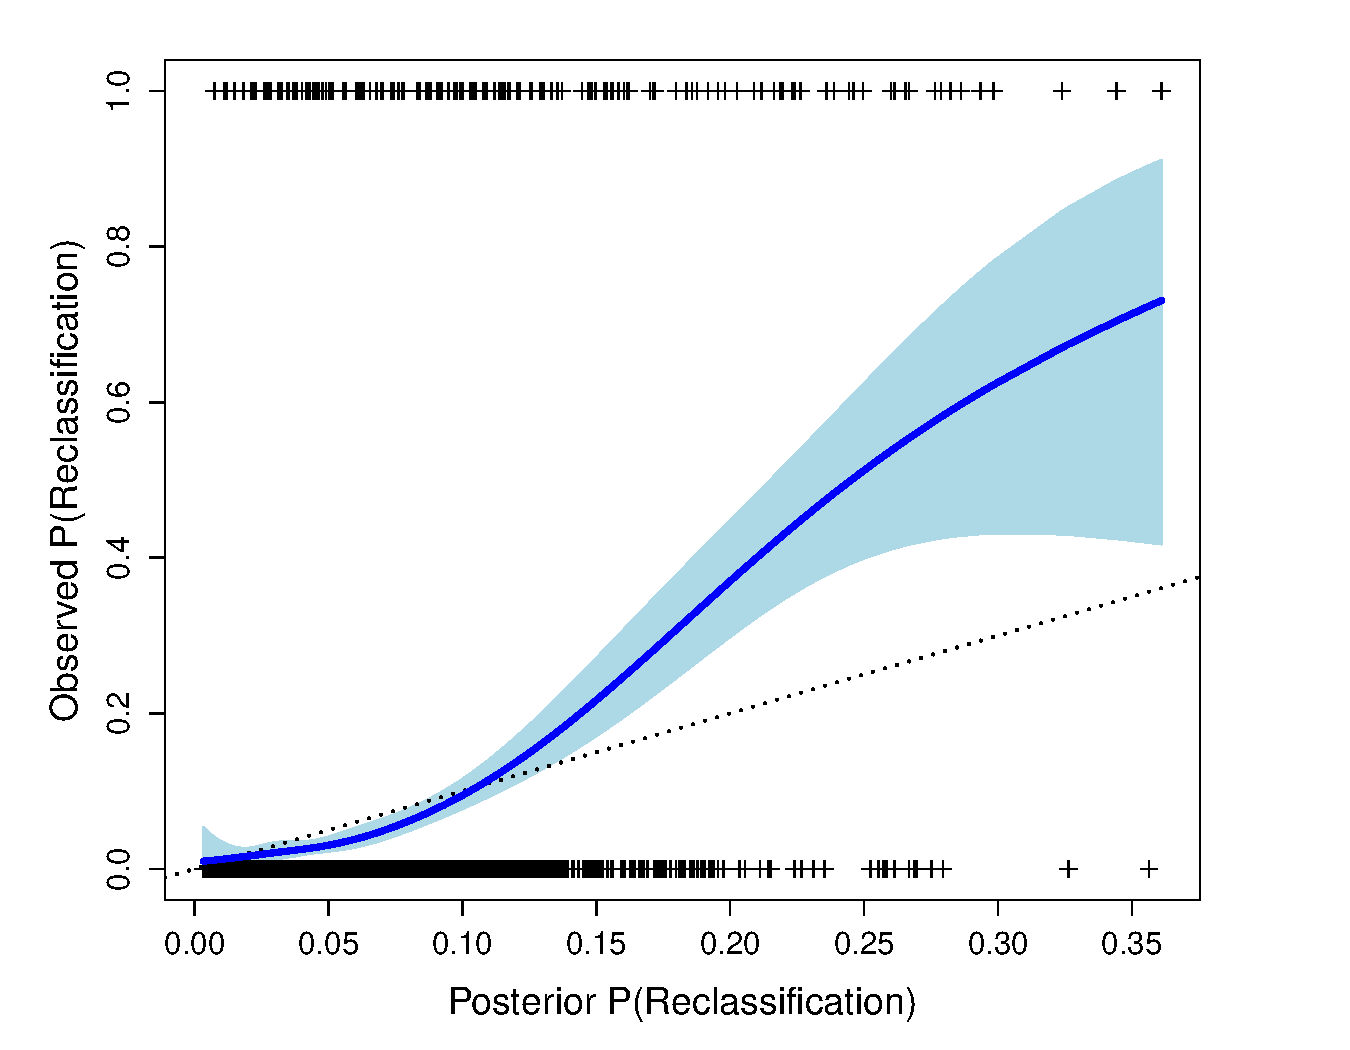
\includegraphics[width=\textwidth]{pred-vs-obs-rc.pdf}
%\caption{}
%\label{fig:calibrartion-rc}
\end{subfigure}
\begin{subfigure}[b]{0.5\textwidth}
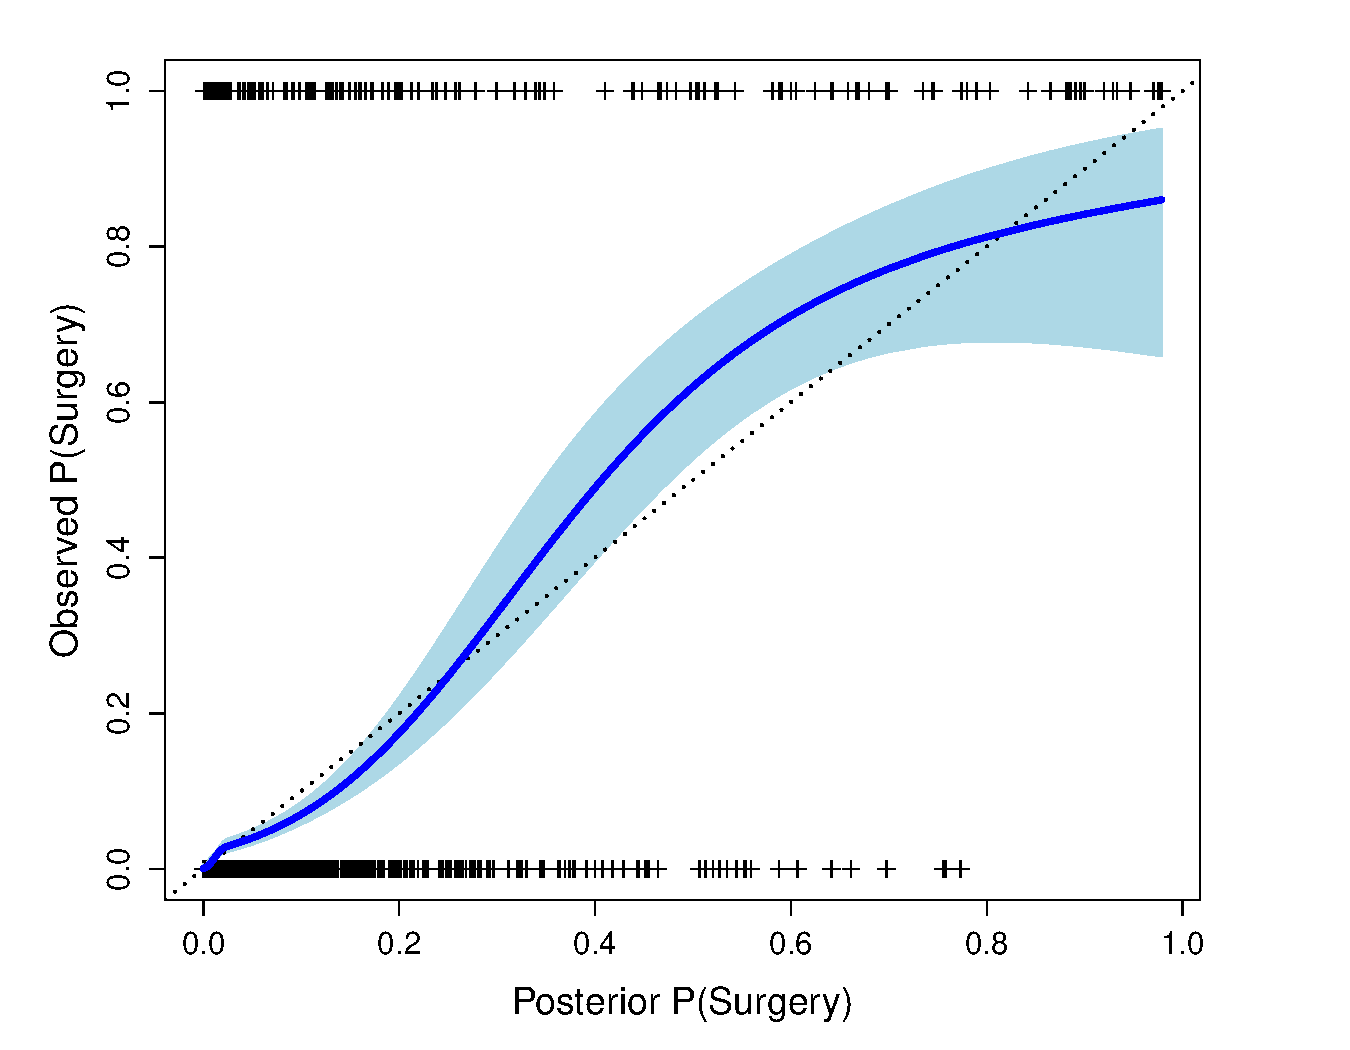
\includegraphics[width=\textwidth]{pred-vs-obs-rrp.pdf}
%\caption{}
%\label{fig:calibrartion-rrp}
\end{subfigure}
\caption{Calibration plots for predicting biopsies (top), reclassification (middle), and surgery (bottom) in annual intervals for all patients} 
\label{fig:calibration-all-bx}
\end{center}
\end{figure}


The model was also fit with informative priors on the effect of partially latent cancer state on the risk of surgery in order to assess robustness of posterior predictions to prior specification and under the concern that the relationship between an outcome's missingness and its value may not be identifiable from the likelihood alone. A range of informative priors (e.g., aggressive cancer increases, does not affect, or decreases risk of surgery) were found to have no impact on the model's predictive accuracy. (For this reason, results are not discussed here in more detail.) Informative priors were not explored for other model parameters as non-indentifiability was not suspected. %which section to put this in?


%%put in all the graphs

\section{Fast, individualized posterior estimates for new data}
In order for the proposed prediction model to be useful in a clinical setting, it is necessary to be able to update posterior estimates quickly  to incorporate new biopsy or PSA results during a patient's visit. While a standard implementation of the proposed model would entail re-running MCMC to obtain updated posteriors of patient-specific variables, this approach could take hours to complete. Instead, we use importance sampling \cite{Bishop2006} to get fast prediction updates. After obtaining posterior estimates using current data, importance sampling to update these estimates for either a new patient or new data on an existing patient requires three steps: generating proposal values for the latent variables to be updated, calculating weights for proposed values, and weighting proposed values to estimate an updated posterior.

In order to generate proposal values for importance sampling for new patients without previous predictions, we start with samples of population-level parameters from the full joint posterior (Equation \ref{eq:post-inf}) based on previously observed data. Then, for each draw, we generate proposed values for patient-specific latent variables (true state, $\eta$, and random effects, $\bmb$) from their conditional posteriors. For patients with existing predictions that only need to be updated, posterior samples of latent variables based on earlier observations can be used as proposal values. Next, the importance weights for proposed values are proportional to the conditional likelihood of all patient data given population-level parameters and proposed latent variables. The weighted proposal distribution then constitutes the updated posterior for patient-specific latent variables. This particular importance sampling procedure can be more specifically described as a one-step version of a sequential importance resampler, also known as a particle filter \cite{Bishop2006}. We give further details of the proposed particle filter in the Appendix. Accompanying code is available at \texttt{http://github.com/rycoley/XXX}.


For implementation in clinical practice, proposals for new patients can be re-generated prior to actually observing new data, so that only weight calculating and re-weighting of the proposal distribution needs to be done in real-time. Then, predictions for each patient can be obtained in a matter of seconds. By random chance, some patients will have data such that very few of the pre-generated proposed latent values will receive high weights; this can cause instability in posterior means. However, such scenarios can be detected by monitoring the effective size of the posterior sample, also known as the effective number of particles. When this number drops below a pre-specified threshold (e.g., 500), the procedure can be repeated with a larger set of pre-generated proposals. 

The proposed importance sampling approach still requires the periodic use of MCMC to perform full model updates, similar to the procedure described in Lee and Chia (2002)\nocite{Lee2002}. While fully online updating of all posteriors (that is, updating not dependent on periodic MCMC) via sequential importance resampling would be ideal, such online methods are known to suffer from the problem of degeneracy when the model includes static parameters (such as the population-level parameters in our model), as explained in Andrieu et al. (2005, section II)\nocite{Andrieu2005}.


\subsection{Application to clinical data}
We assessed performance of the proposed importance sampling approach in the Johns Hopkins Active Surveillance cohort data. We compared the posterior probability of aggressive cancer, $P(\eta_i)$, obtained from MCMC performed in \texttt{JAGS} under two scenarios for each patient in the cohort without true cancer state observed. First, we examine agreement between the two models when each patient is completely new, that is, MCMC is performed in the absence of any of their data and, then, the particle filter is used to predict their true cancer using all of their available data. Second, we consider the scenario where additional data is observed for a patient who has already been included in the prediction model. Specifically, MCMC is performed including all data from a patient up until their penultimate biopsy (and all data from all other patients). Then, the particle filter is used to predict their true cancer state using the remaining data for that patient. 

Results of this comparison are shown in Figure \ref{fig:jags-vs-pf}. On the left, we see agreement between methods when a patient is newly introduced. Here, correlation between posterior probabilities from \texttt{JAGS} and the particle filter is 0.9950. The righthand panel compares posterior predictions between the \texttt{JAGS} fit and the particle filter for each patient when the final biopsy is included. In this scenario, the correlation is 0.XX. From these results, we conclude that the particle filter is an appropriate substitute for full MCMC runs in order to provide real-time updates in a clinical setting. 

\begin{figure}
\begin{center}
\begin{subfigure}[b]{0.45\textwidth}
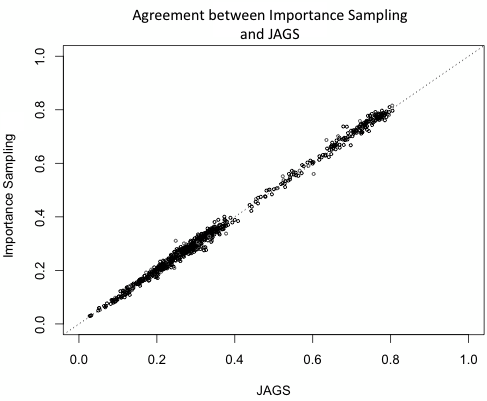
\includegraphics[width=\textwidth]{2015-07-01_compare_fits_manual-edit}
\end{subfigure}
\begin{subfigure}[b]{0.45\textwidth}
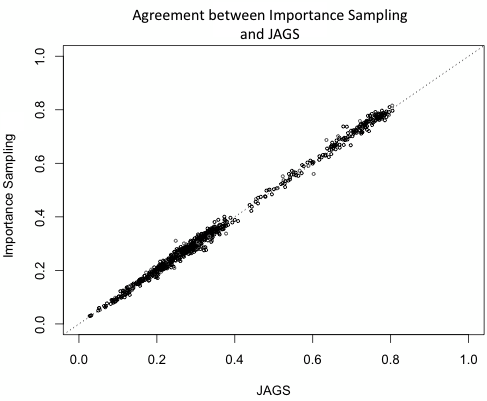
\includegraphics[width=\textwidth]{2015-07-01_compare_fits_manual-edit}
\end{subfigure}
\caption{Agreement between importance sampling and JAGS posterior predictions of prostate cancer state for a new patient (left panel) and for a patient with updated data (right panel). (Placeholder figures) }
\label{fig:jags-vs-pf}
\end{center}
\end{figure}


\section{Discussion}
In this paper, we have presented a hierarchical Bayesian joint model for predicting latent cancer state among low risk prostate cancer patients. While many models exist for providing individualized predictions of biopsy results for this population, ours is the first model to propose prediction of the outcome of chief concern- the true underlying state of an individual's prostate cancer. This model demonstrates the potential for new precision medicine approaches that provide individualized predictions of latent health states and trajectories, instead of focusing only on error-prone measurements of the health state. 
%Within a hierarchical latent class framework, our model also predicts likely outcomes of biopsy and PSA tests, which can guide decision-making about future tests.

The proposed prediction model also exemplifies the statistical underpinnings of a learning health care system \cite{Smith2013}. As more patients enroll in the Johns Hopkins Active Surveillance cohort, and as more information is collected on existing patients, our ability to predict underlying health states and the likely trajectory of clinical outcomes improves. Through a real-time importance sampling algorithm, updated predictions based on the most current information can be communicated to patients in a clinical setting to support decision making. At this time, real-time updating is only available for individual-level parameters; standard Bayesian estimation procedures can be routinely performed on refreshed data to update all  model hyperparameters. Further research on cutting edge alternative methods (see Kantas et al. (2014)\nocite{Kantas2014}) will enable us to support fully online updating in the future.  

As is typical in applied work, this model is limited by the assumptions it involves. In particular, we assume that an individual's latent cancer state is constant during surveillance. The bias introduced by this assumption is likely small, as Porten et al. (2011)\nocite{Porten2011} show that upgrading, particularly early on in active surveillance, is likely due to misclassification at diagnosis rather than tumor dedifferentiation. Moreover, the implications of previous research on the rate of progression among men with low risk diagnoses are limited because a distinction between progression of the underlying cancer state and missed diagnoses due to sampling error was notably absent \cite{Tseng2010}. More recently, however, Inoue et al. (2014), using a natural history approach to modeling the rate of disease progression that also accounted for the error of biopsy grading, estimated a 12-24$\%$ rate of disease progression rate within ten years of enrollment among the Johns Hopkins AS cohort. In light of this research, we intend to extend this model to allow for time-varying health state. %\textit{I think I need a better response than this!}
%Consistent with this assumption is the belief held by many clinicians that reclassification during active surveillance is due primarily to under-diagnosis at earlier biopsies. Furthermore, Author (Year) found little evidence of de-differentiation in low risk cancer patients, but a more recent examination by Inoue et al. (2014) brings this conclusion into question. 

Other assumptions in this model can be easily modified in response to the availability of additional data or an evolution in scientific understanding including, for example, the assumption of a shared covariance matrix for random effects across latent states. Moreover, this model can easily accommodate new predictors or outcomes. If, for example, a genetic marker for prostate cancer risk were identified, the probability distribution for latent state could be stratified by subgroups defined by this marker. Or, if additional biopsy results, such as the number of positive cores or maximum percent cancer involvement, were thought to be predictive of true cancer state, regressions of these repeated outcome measures on latent class could also be included in the joint model. (These outcomes were not associated with cancer state in our cohort and, as a result, were not included in the proposed model.) This ability to update the prediction model based on data availability and clinical expertise further reflects the characteristics of a learning health care system. 


\bibliographystyle{plain}
\bibliography{/Users/ryc/Dropbox/inhealth/inhealth-bib}

\section{Appendix}
\subsection{Importance sampling procedure}
For the purposes of this appendix, we introduce the following abbreviated form of the joint posterior given in \ref{eq:post-inf}: 
\begin{equation}
p(\theta,b_{1:n}|y_{1:n})\propto\prod_{i=1}^{n}[f(y_{i}|b_{i},\theta)g(b_{i}|\theta)]\pi(\theta)\label{eq:posterior_n}
\end{equation}
 Where $y_{i}$ is the vector of measurements for patient $i$, $y_{1:n}$ is the list of measurements for the first $n$ patients, $b_{i}$ is a vector of latent variables for patient $i$, $b_{1:n}$ is a list of latent variables for the first $n$ patients, $\theta$ contains the population-level parameters, $\pi$ is the prior for $\theta$, and $f$ and $g$ are multivariate distributions coming from the model likelihood in \ref{eq:lik-inf}. We first illustrate how importance weighting can be used to quickly estimate latent variables for a new patient before showing how similar calculations can be done to incorporate newly measured data on existing patients in real-time.
 
\subsubsection{Fast predictions for a new patient}
 Here, we focus on obtaining posteriors of latent variables for a new patient (indexed by $n+1$). Our ultimate goal is to calculate expectations with respect to the posterior distribution based on all $n+1$ patients (i.e. $p(\theta,b_{1:(n+1)}|y_{1:(n+1)})$). While we cannot immediately draw from this distribution, we can evaluate a function that is proportional to its density (Equation \ref{eq:posterior_n}). To carry out importance sampling, we need to choose a proposal distribution $q$ from which to generate candidate values of $(\theta,b_{1:(n+1)})$. We use the posterior distribution based on the first $n$ patients as our proposal distribution. This approach is analogous to a one-step particle filter \cite{Bishop2006}.
\begin{eqnarray*}
q(\theta,b_{1:(n+1)}) & := & g(b_{n+1}|\theta)p(\theta,b_{1:n}|y_{1:n})
\end{eqnarray*}

Practically, this consists of taking $J$ draws of $\theta$ and $b_{1:n}$ from the previously fitted posterior in Eq \ref{eq:posterior_n}. Then, conditional on $\theta$, we draw $b_{n+1}$ from the distribution $g$. We index each of the resulting draws as $(\theta^{(j)},b_{1:(n+1)}^{(j)})$, with $j=1,\dots,J$. The importance weights $w_{j}$ are then proportional to 
\begin{eqnarray}
w^{(j)} & \propto & \frac{p(\theta^{(j)},b_{1:(n+1)}^{(j)}|y_{1:(n+1)})}{q(\theta^{(j)},b_{1:(n+1)}^{(j)})} \nonumber \\
 & \propto & \frac{\prod_{i=1}^{n+1}[f(y_{i}|b_{i}^{(j)},\theta^{(j)})g(b_{i}^{(j)}|\theta^{(j)})]\pi(\theta^{(j)})}{g(b_{n+1}^{(j)}|\theta^{(j)})\prod_{i=1}^{n}[f(y_{i}|b_{i}^{(j)},\theta^{(j)})g(b_{i}|\theta^{(j)})]\pi(\theta^{(j)})} \nonumber \\
\label{eq:importance-weights}
 & = & f(y_{i}|b_{i}^{(j)},\theta^{(j)})
\end{eqnarray}

The final weights $w^{(j)}$ are standardized to sum to 1. The new posterior for $(\theta,b_{1:(n+1)})$ can then be represented as the mixture distribution satisfying $P(\theta=\theta^{(j)},b_{1:(n+1)}=b_{1:(n+1)}^{(j)})=w^{(j)}$. A posterior mean for $b_{(n+1)}$ can be calculated as $\sum_{j=1}^{J}w^{(j)}b_{(n+1)}^{(j)}$. The unstandardized weights can also be used in a rejection sampling procedure, although we found this approach to be less computationally efficient than importance sampling for our scenario.


\subsubsection{Fast predictions for existing patients with new data}

For a patient $k$ with existing data, where we already have a posterior sample for their latent variable values, we instead use this posterior as our proposal distribution $q(\theta^{(j)},b_{1:n}^{(j)})$, with $i\leq n$. Let $y_{1:n}^{k+}$ refer to the data set after incorporating new data on patient $k$, where $y_{i}^{+}=y_{i}$ if $k\neq i$. The importance weights in Equation \ref{eq:importance-weights} then simplify to
\begin{eqnarray*}
w^{(j)} & \propto & \frac{p(\theta^{(j)},b_{1:n}^{(j)}|y_{1:n}^{+})}{q(\theta^{(j)},b_{1:n}^{(j)})}\\
 & \propto & \frac{\prod_{i=1}^{n}[f(\ensuremath{y_{i}^{+}}|b_{i}^{(j)},\theta^{(j)})g(b_{i}^{(j)}|\theta^{(j)})]\pi(\theta^{(j)})}{\prod_{i=1}^{n}[f(\ensuremath{ y_{i} }|b_{i}^{(j)},\theta^{(j)})g(b_{i}^{(j)}|\theta^{(j)})]\pi(\theta^{(j)})}\\
 & = & \frac{f(\ensuremath{ y_{k}^{+}} |b_{ k }^{(j)},\theta^{(j)})}{f(\ensuremath{ y_{k}} |b_{k}^{(j)},\theta^{(j)})}
\end{eqnarray*}

Let $L_{k}$ denote that number of measurements for which we've previously fit a posterior for $b_{k}$, and let $N_{k}$ denote the number of new measurements we wish to incorporate into this posterior. Then, $y_{k}^{+}$ can be expressed as the vector $y_{k}^{+}=(y_{k[1]},y_{k[2]},\dots y_{k[L_{k}]},y_{k[L_{k}+1]}^{+},\dots y_{k[L_{k}+N_{k}]}^{+})$, where $y_{k[l]}^{+}$ is the $l^{th}$ measurement from patient $k$. If the repeated measures for each patient are independent conditional on $b_{i}$, as is the case in the proposed model, then the above ratio reduces to

\begin{eqnarray*}
w^{(j)} & \propto & \frac{\prod_{l=1}^{L_{k}+N_{k}}f(\ensuremath{ y_{k[l]}^{+}} |b_{k}^{(j)},\theta^{(j)})}{\prod_{l=1}^{L_{i}}f(\ensuremath{y_{k[l]}} |b_{ k}^{(j)},\theta^{(j)})}\\
 & = & \prod_{l=L_{k}+1}^{L_{k}+N_{k}}f(\ensuremath{y_{k[l]}^{+}}|b_{k}^{(j)},\theta^{(j)})
\end{eqnarray*}


We then proceed as above to get a re-weighted posterior for the latent variables of patient $k$. 


\end{document}
